\documentclass[a4paper,12pt]{article}

% include headers and preamble for reoport
% file: includes-report.tex
% -----------------------------------------------------------------------------
% includes for studies report
% -----------------------------------------------------------------------------

\usepackage{amsmath}
\usepackage{setspace}
\usepackage[top=1.2in, bottom=1.2in]{geometry}
\usepackage[x11names]{xcolor}

\usepackage{float} % to force placement of images etc.

\usepackage{graphicx}
\usepackage[utf8]{inputenc}
\usepackage{siunitx}

% // -- for different section heading color --
\usepackage{sectsty}
\usepackage{xcolor}
% \chapterfont{\color{blue}}  % sets colour of chapters
% \definecolor{MyBlue}{rgb}{0.78,0.9,1} % rgb color code
% \definecolor{DarkBlue}{HTML}{002f4c} % HTML HEX color code
\definecolor{DarkBlue}{RGB}{0,47,76} % RGB color code
\sectionfont{\color{DarkBlue}}  % sets colour of sections
\subsectionfont{\color{DarkBlue}}  % sets colour of sections

\usepackage{float}


%\usepackage{multirow}
%\usepackage{pgfplots}
\usepackage{subcaption}

% // -- for source code listings --
\usepackage{color}
\definecolor{OliveGreen}{RGB}{0,128,0}
\usepackage{listings}
\usepackage{caption}
\DeclareCaptionFont{white}{\color{white}}
\DeclareCaptionFormat{listing}{\colorbox{gray}{\parbox{\textwidth}{#1#2#3}}}
\captionsetup[lstlisting]{format=listing,labelfont=white,textfont=white}


\lstdefinestyle{cStyle}{language=C}
\lstset{
language=C,
%basicstyle=\small\ttfamily,
basicstyle=\small\ttfamily,
keywordstyle=\color{blue}\ttfamily,
stringstyle=\color{red}\ttfamily,
commentstyle=\color{magenta}\ttfamily,
morecomment=[l][\color{magenta}]{\#},
numbers=left,
numberstyle=\tiny,
% frame=tb,
columns=fullflexible,
showstringspaces=false,
tabsize=2
}
\usepackage{matlab-prettifier}
\lstdefinestyle{matlabStyle}{language=matlab}
\lstset{
%style=Matlab-editor,
language=matlab,
%basicstyle=\small\ttfamily,
basicstyle=\small\ttfamily,
keywordstyle=\color{blue}\ttfamily,
stringstyle=\color{red}\ttfamily,
commentstyle=\color{OliveGreen}\ttfamily,
morecomment=[l][\color{OliveGreen}]{\#},
numbers=left,
numberstyle=\tiny,
% frame=tb,
columns=fullflexible,
showstringspaces=false,
tabsize=2
}
\lstdefinestyle{vhdlStyle}{language=vhdl}
\lstset{
language=vhdl,
%basicstyle=\small\ttfamily,
basicstyle=\small\ttfamily,
keywordstyle=\color{blue}\ttfamily,
stringstyle=\color{red}\ttfamily,
commentstyle=\color{magenta}\ttfamily,
morecomment=[l][\color{magenta}]{\#},
numbers=left,
numberstyle=\tiny,
% frame=tb,
columns=fullflexible,
showstringspaces=false,
tabsize=2
}

% bibliography (Literaturverzeinis)
\usepackage[round]{natbib}
\bibliographystyle{alphadin} % set format

% // -- source code listings --


\title{Bachelorprojekt}
\date{2018-11-21}
\author{Fabian Huber}

\begin{document}

% Titlepage for HAW lab report
\begin{titlepage}
\definecolor{blue(ncs)}{rgb}{0.0, 0.53, 0.74}
\begin{figure}[h!]
  \begin{flushright}
  \begin{spacing}{1.5}
  
\includegraphics[width=.5\linewidth]{images/hawlogo.png}
  \label{fig:hawlogo}\\
  \small Fakultät Technik und Informatik\\
  \small Department Informations- und Elektrotechnik
  \end{spacing}
  \end{flushright}
\end{figure}
\textbf{\large Bachelorprojekt}
\begin{center}\noindent\textcolor{blue(ncs)}{\rule{13.5cm}{0.5mm}}\end{center}
\begin{spacing}{4.5}
\textbf{\huge Automated Driving}
\end{spacing}
\textbf{\large\indent RC Car Control with Open Source Image Processing}
\begin{center}\noindent\textcolor{blue(ncs)}{\rule{13.5cm}{0.5mm}}\end{center}
\begin{spacing}{1.15}
\vspace*{\fill}
\noindent
\textnormal{\\
  Prof. Dr.-Ing. Marc Hensel \\
  \textbf{Projektgruppe:} Fabian Huber, Enzo Morino, Markus Trockel \\
  \textbf{Abgabe:} 11.02.2019 \\
}
\end{spacing}
\end{titlepage}
% --- end of titlepage ---

  \pagenumbering{gobble}

	% --- Abstract/Kurzübersicht ---
	\newpage
	\section*{Kurzübersicht}
Das Ziel des Projekts ist ein Modellauto, das mit Kamera, Abstandssensor und
Rapsberry Pi ausgestattet, durch Fahrbahnlinienerkennung teilautonom einem
Straßenverlauf foglen kann. Es ist eine pratkitsche Umsetzung von Systemarchitektur, Sensorik und der Nutzung von den Werkzeugen der Bildverabreitung der Library openCV in Python.\\
Dafür ist ein Prozess entwickelt worden, bei dem aus Sensordaten
Steuerungsinformationen für den Wagen generiert werden. Die Durchführung hat
gezeigt, dass die Umsetzung möglich ist, dass für eine stabile Funktionsweise
weitere Entwicklungen von Funktionen nötig sind, die die zeitkritischen
Anforderungen erfüllen und hardwarebedingte Fehleranfälligkeiten abfangen, um so
eine rkontinuierliche Fahrt zu ermöglichen.\\

	
	% --- Inhaltsverzeichnis ---
  \newpage
  \tableofcontents
  \newpage

  \pagenumbering{arabic}



% --- Kapitel ---
	\newpage
  \section{Einleitung}
Im Jahr 2005 ging das Projektauto Stanley der Standford University an den Start
der DARPA Grand Challenge, einem Rennen autonomer Fahrezeuge über eine
definierte Strecke in der Mojave-Wüste. Nach 212,76km durch unwegsames Gelände
ging Stanley als Erster über die Ziellinie und das Team um Professor Sebastian
Thrun war Gewinner des mit 2 Millionen Dollar dotierten Rennens.\\
Die Entwicklung des autonomen Fahrens für Fahrzeuge des Straßenverkehrs ist ein
aktuelles Thema, das immer mehr in die Praxis umgesetzt wird. Dabei gibt es
verschiedenen Stufen des teilautonomen Fahrens. So gehört zur Stufe 2 die
Funktion, dass Lenkvorgänge vom Fahrassistenten ausgeführt werden.\\
Durch dieses Projekts soll ein Einblick in die Materie geschaffen
werden und die Umsetzbarkeit im Rahmen studentischer Möglichkeiten erfahren
werden.\\
Die Autoren wollen mit ihrem Auto Hawey einen Startschuß setzen und mit diesem
Bericht ein nachfolgendes Team inhaltlich in der Sache abholen, dass ein
Einstieg in das Projekt und so ein konstruktives Fortsetzten und Verbessern 
möglich ist.\\

Fabian Huber, Enzo Morino, Markus Trockel

 
 	\newpage
  \section{Ziel des Projekts}
Das Projekt hat als Ziel, ein Modellauto mit Elektroantrieb 
durch Fahrbahnlinienerkennung eine vorgegebene Strecke fahren zu lassen. Als
technische Bestandteile wird ein Raspberry Pi 3 mit dazugehöriger Kamera
gewählt, dazu ein Sensor zur Abstandsmessung, um etwaige Kollisionen zu
vermeiden. Implementiert wird der Code in Python unter der Nutzung der
Bildverarbeitungslibrary openbCV. \\
Das Auto soll  sowohl ein 4m lange Strecke gradeaus als auch in Kurven von 90° 
zwischen zwei Fahrbahnlinien die Spur halten. Idealerweise ist es möglich, dass 
der Wagen auch mit Linienunterbrechungen weitersteuern und so eine acht-förmige 
Strecke abfahren kann wie sie beim Carolo-Cup, einem Wettbewerb für autonome
Modellfahrzeuge, befahren wird.


  \newpage  
  \section{Prinzip der Steuerung} 	
  Über ein Python-Programm, welches auf dem Raspberry Pi läuft, wird der Video-Stream der angeschlossenen Kamera iterativ ausgewertet. Es werden die beiden Fahrbahnlinien erkannt, durch Geraden angenähert und deren Fluchtpunkt berechnet. Auf Grundlage der x-Koordinate dieses Fluchtpunktes wird ein Ausgangssignal berechnet, welches über das PWM-Modul den Servo ansteuert, und damit den Lenkwinkel festlegt.  


  \section{Hardware}
  Für die technische Umsetzung werden eine Reihe von Komponenten verwendet.

  \subsection{Raspberry Pi 3}
  
    % image of the raspberry pi - source: http://www.raspberrypi.org
    \begin{minipage}{\columnwidth}
      \makeatletter
      \def\@captype{figure}
      \makeatother
      \centering
      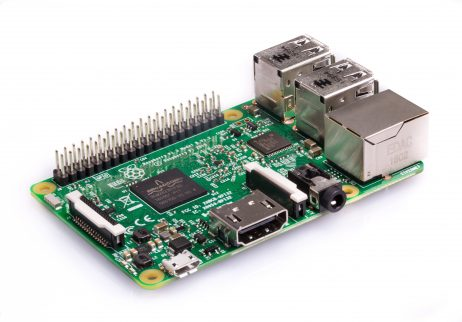
\includegraphics[width=0.6\linewidth]{images/hw_raspberrypi3.jpg}
      \caption{Raspberry Pi 3 Model B}
      \label{fig:img-hw-01}
    \end{minipage}
    \vspace{1cm}

    \noindent
    Das Herzstück des Projekts bildet ein Raspberry Pi 3 Model B. Ausgestattet
    ist dieser Mini-PC neben den üblichen Schnittstellen mit drei Elementen, die
    für das Vorhaben essentiell sind: Einem Wifi Modul, einem Ethernet-Port und
    allem einem GPIO Header mit reichlich freien Pins.\\
    \ \\
    Als Betriebssystem nutzt der Raspberry Pi das hauseigene Debian Derivat
    Raspbian. \\

  \subsection{Motorcontroller}

    % image of the motor and servo controller module  - source: https://www.makerlab-electronics.com
    \begin{minipage}{\columnwidth}
      \makeatletter
      \def\@captype{figure}
      \makeatother
      \centering
      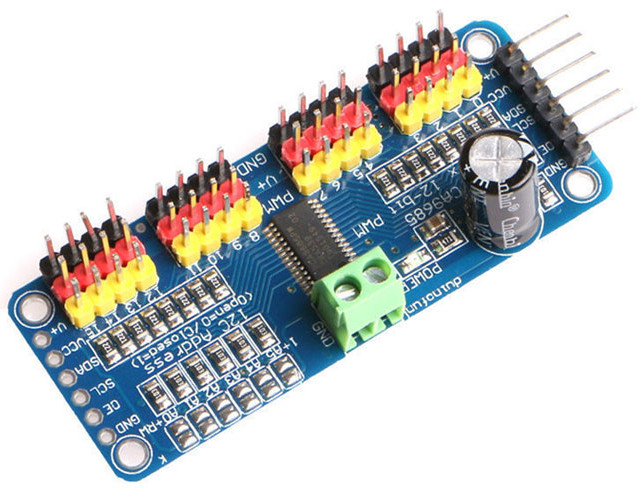
\includegraphics[width=0.4\linewidth]{images/hw_pca9685.jpg}
      \caption{PCA9685 Controller Modul}
      \label{fig:img-hw-02}
    \end{minipage}
    \vspace{1cm}

    \noindent
    Der Fahrtenregler des Motors für den Antrieb und der Servo für die Lenkung
    des RC Fahrzeugs werden über das PCA9685 Controller Modul mittels
    Pulsweitenmodulation angesprochen. Die Implementierung selbst ist
    glücklicherweise bereits durch eine offene Python Bibliothek (siehe Tab.
    \ref{tab:sw-01}) verfügbar. 
  
  \subsection{Raspberry Pi Camera Module}
    % image of the camera module - source: https://www.raspberrypi.org
    \begin{minipage}{\columnwidth}
      \makeatletter
      \def\@captype{figure}
      \makeatother
      \centering
      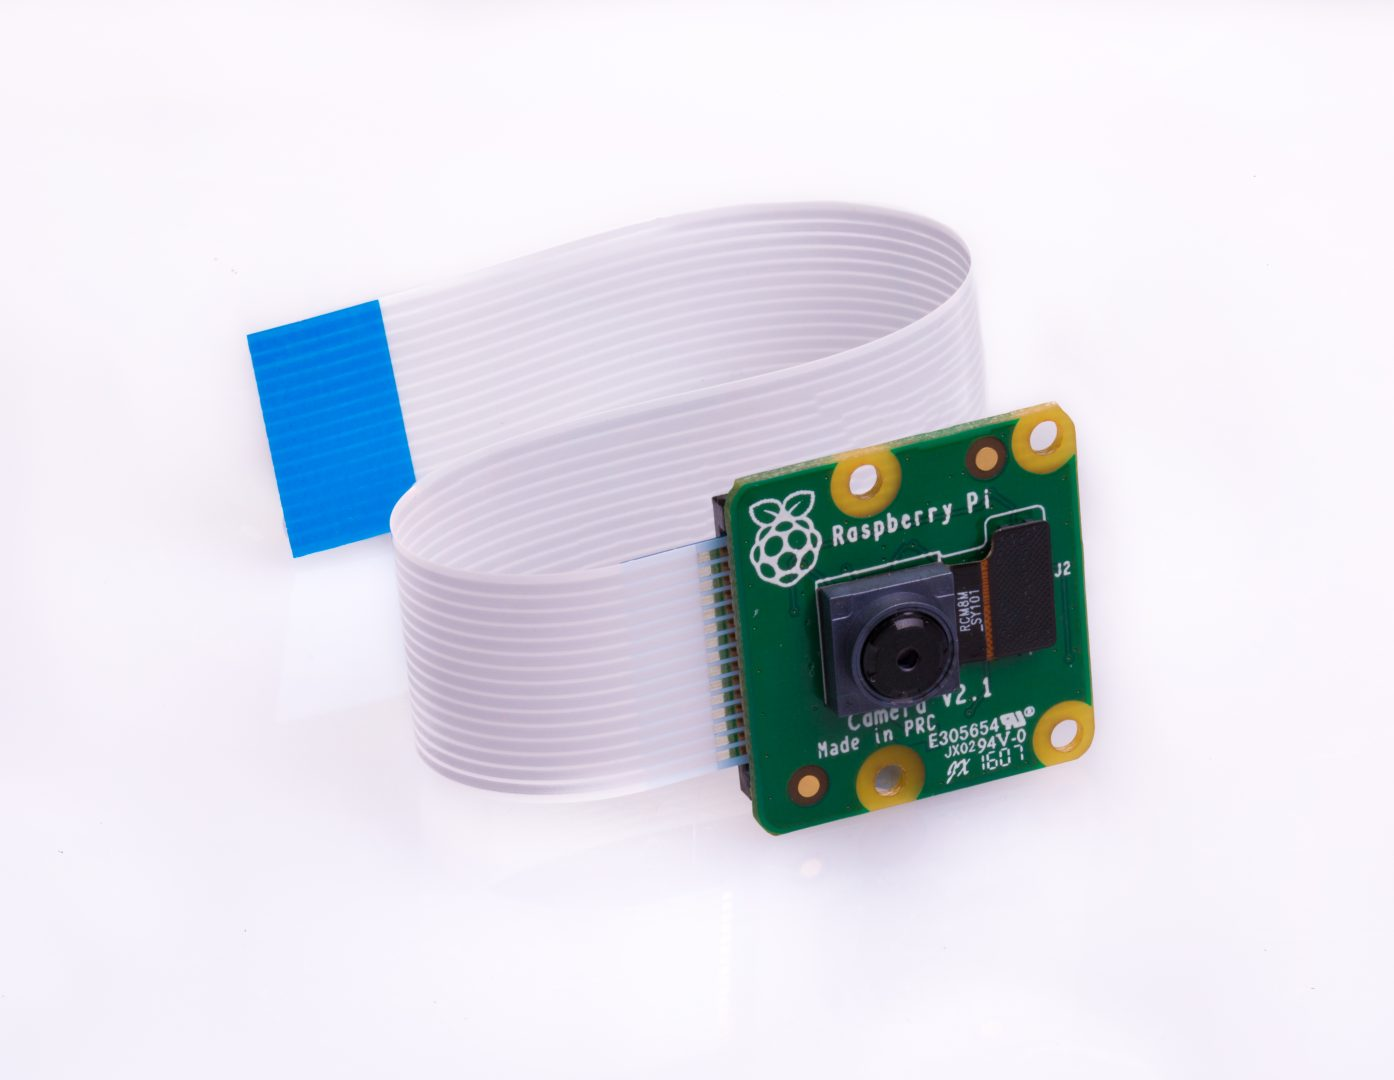
\includegraphics[width=0.6\linewidth]{images/hw_picam.jpg}
      \caption{Camera Module V2}
      \label{fig:img-hw-03}
    \end{minipage}
    \vspace{1cm}

    \noindent
    Das Sehen ermöglicht das eingesetzte Raspberry Pi Kameramodul, welches über
    einen speziell am Raspberry Pi vorhandenen Kameraanschluss. Verbaut ist
    ein Sony IMX219 8-Megapixel Sensor der ebenfalls direkt über vorhandene
    Python Bibliotheken performant und resourcenschonend ausgelesen werden kann.

  \subsection{Ultraschallsensor}

    % image of ultrasonic sensor module  - source: https://www.makerfabs.com 
    \begin{figure}[H]
    \center
    \begin{subfigure}{.5\textwidth}
      \centering
      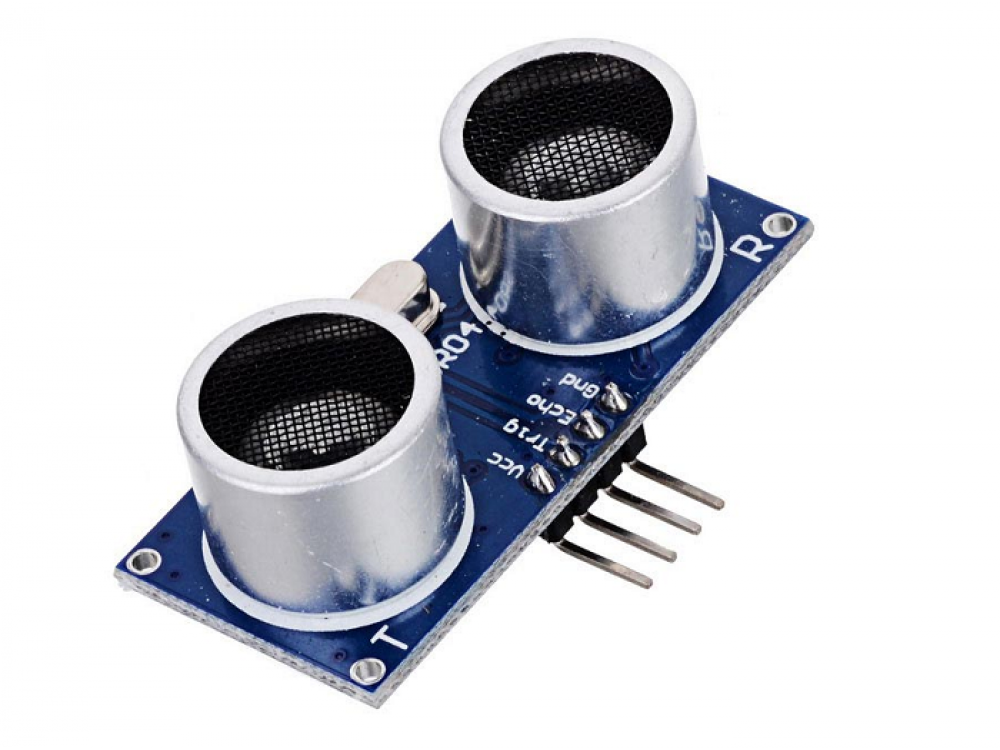
\includegraphics[width=.8\linewidth]{images/hw_hcsr04_01.png}
    \end{subfigure}%
    \begin{subfigure}{.5\textwidth}
      \centering
      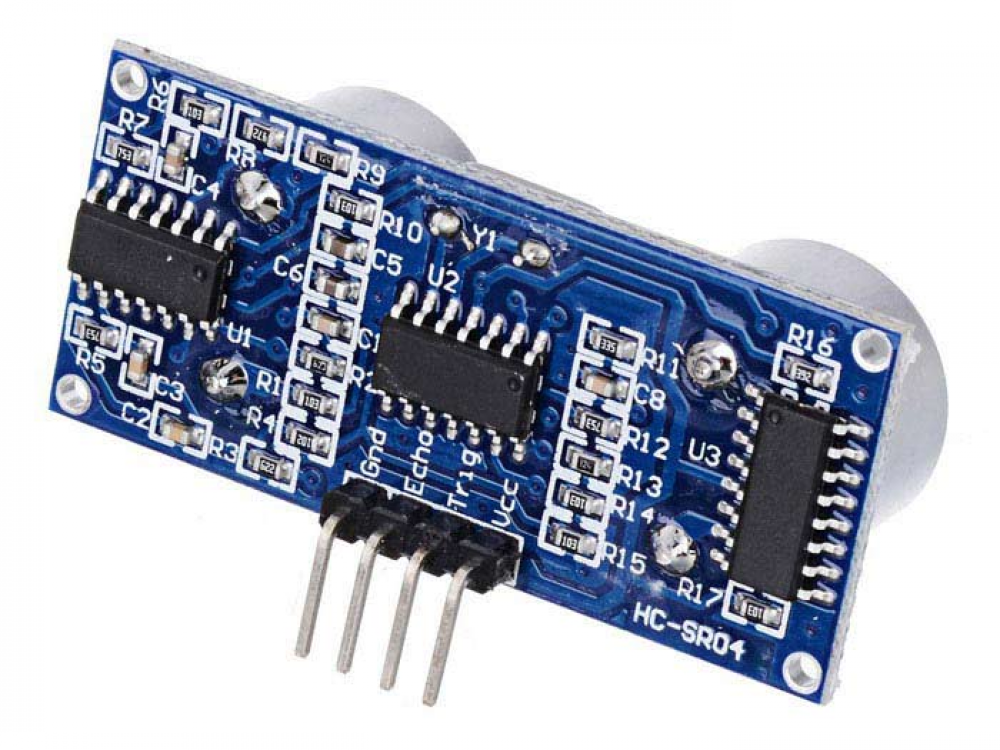
\includegraphics[width=.8\linewidth]{images/hw_hcsr04_02.png}
    \end{subfigure}
      \caption{HC-SR04 Sensor Modul}
      \label{fig:img-hw-04}
    \end{figure}
    \vspace{1cm}
    Im Falle eines anstehenden Frontalzusammenstoßes mit einer Wand oder einem
    anderen größeren Hindernis, soll zusätzlich zur Kamera vorne am Fahrzeug ein
    Ultraschallsensor angebracht werden, der unmittelbare Hindernisse melden
    kann. Hier kommt der HC-SR04 zum Einsatz. Für die Abstandsmessung sendet
    dieser in regelmäßígen Abständen Ultraschallpulse aus und empfängt dann das
    rückgeworfene Echo. Die Laufzeit gibt Auskunft über den Abstand zum
    Hindernis. Fällt dieser Abstand unterhalb eines bestimmten Schwellwerts, so
    wird der Antrieb automatisch gestoppt und keine weiteren Signale
    verarbeitet.

  \subsection{RC Fahrzeug}

    Als Chassi dient ein Einsteiger RC-Modell von dem Elektronik-Versandhandel
    Conrad Electronic. Die mitgelieferten Module für Antrieb und Lenkung können
    ohne Probleme direkt mit dem verwendeten Motorcontroller verwendet werden.
    Einzig der Lenkservo musste zwischenzeitlich durch ein robusteres Modell 
    ausgetauscht werden da er durch einen Fehler in der Programmierung
    übersteuert und damit das Getriebe unbrauchbar wurde. \\
    Der enthaltene Akku kann mithilfe eines einfachen Voltage Regulators
    ebenfalls eingesetzt und zur Stromversorgung des Raspberry Pi verwendet
    werden. \\
    Die Karosserie wird durch einen eigens gefertigten Acrylaufbau ersetzt, der
    mehr Raum für Raspberry Pi und Module bietet und zudem eine stabilen Basis
    für den Kameramast mitbringt.
    \ \\
    % image of the car with setup
    \begin{minipage}{\columnwidth}
      \makeatletter
      \def\@captype{figure}
      \makeatother
      \centering
      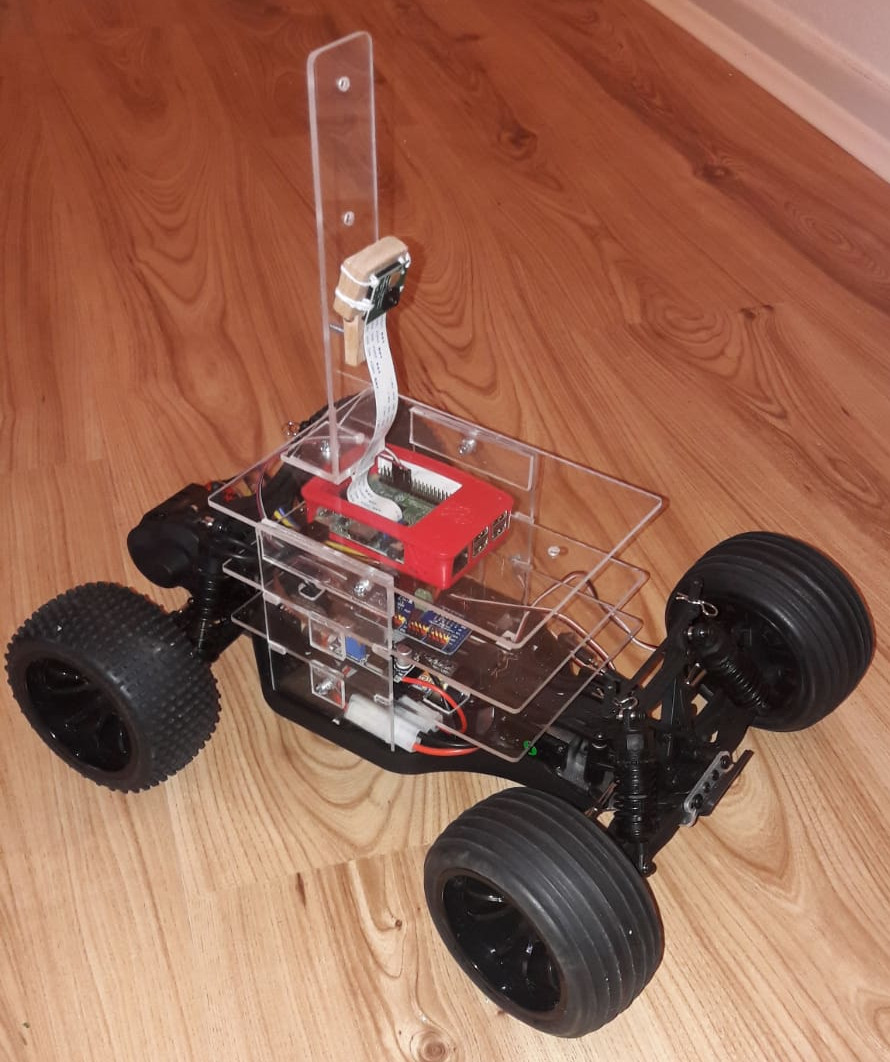
\includegraphics[width=0.6\linewidth]{images/hw_setup.jpg}
      \caption{RC Chassis mit Aufbau}
      \label{fig:img-hw-05}
    \end{minipage}
    \vspace{1cm}

  \subsection{Aufbau}
    % image of the exact setup
    \begin{minipage}{\columnwidth}
      \makeatletter
      \def\@captype{figure}
      \makeatother
      \centering
      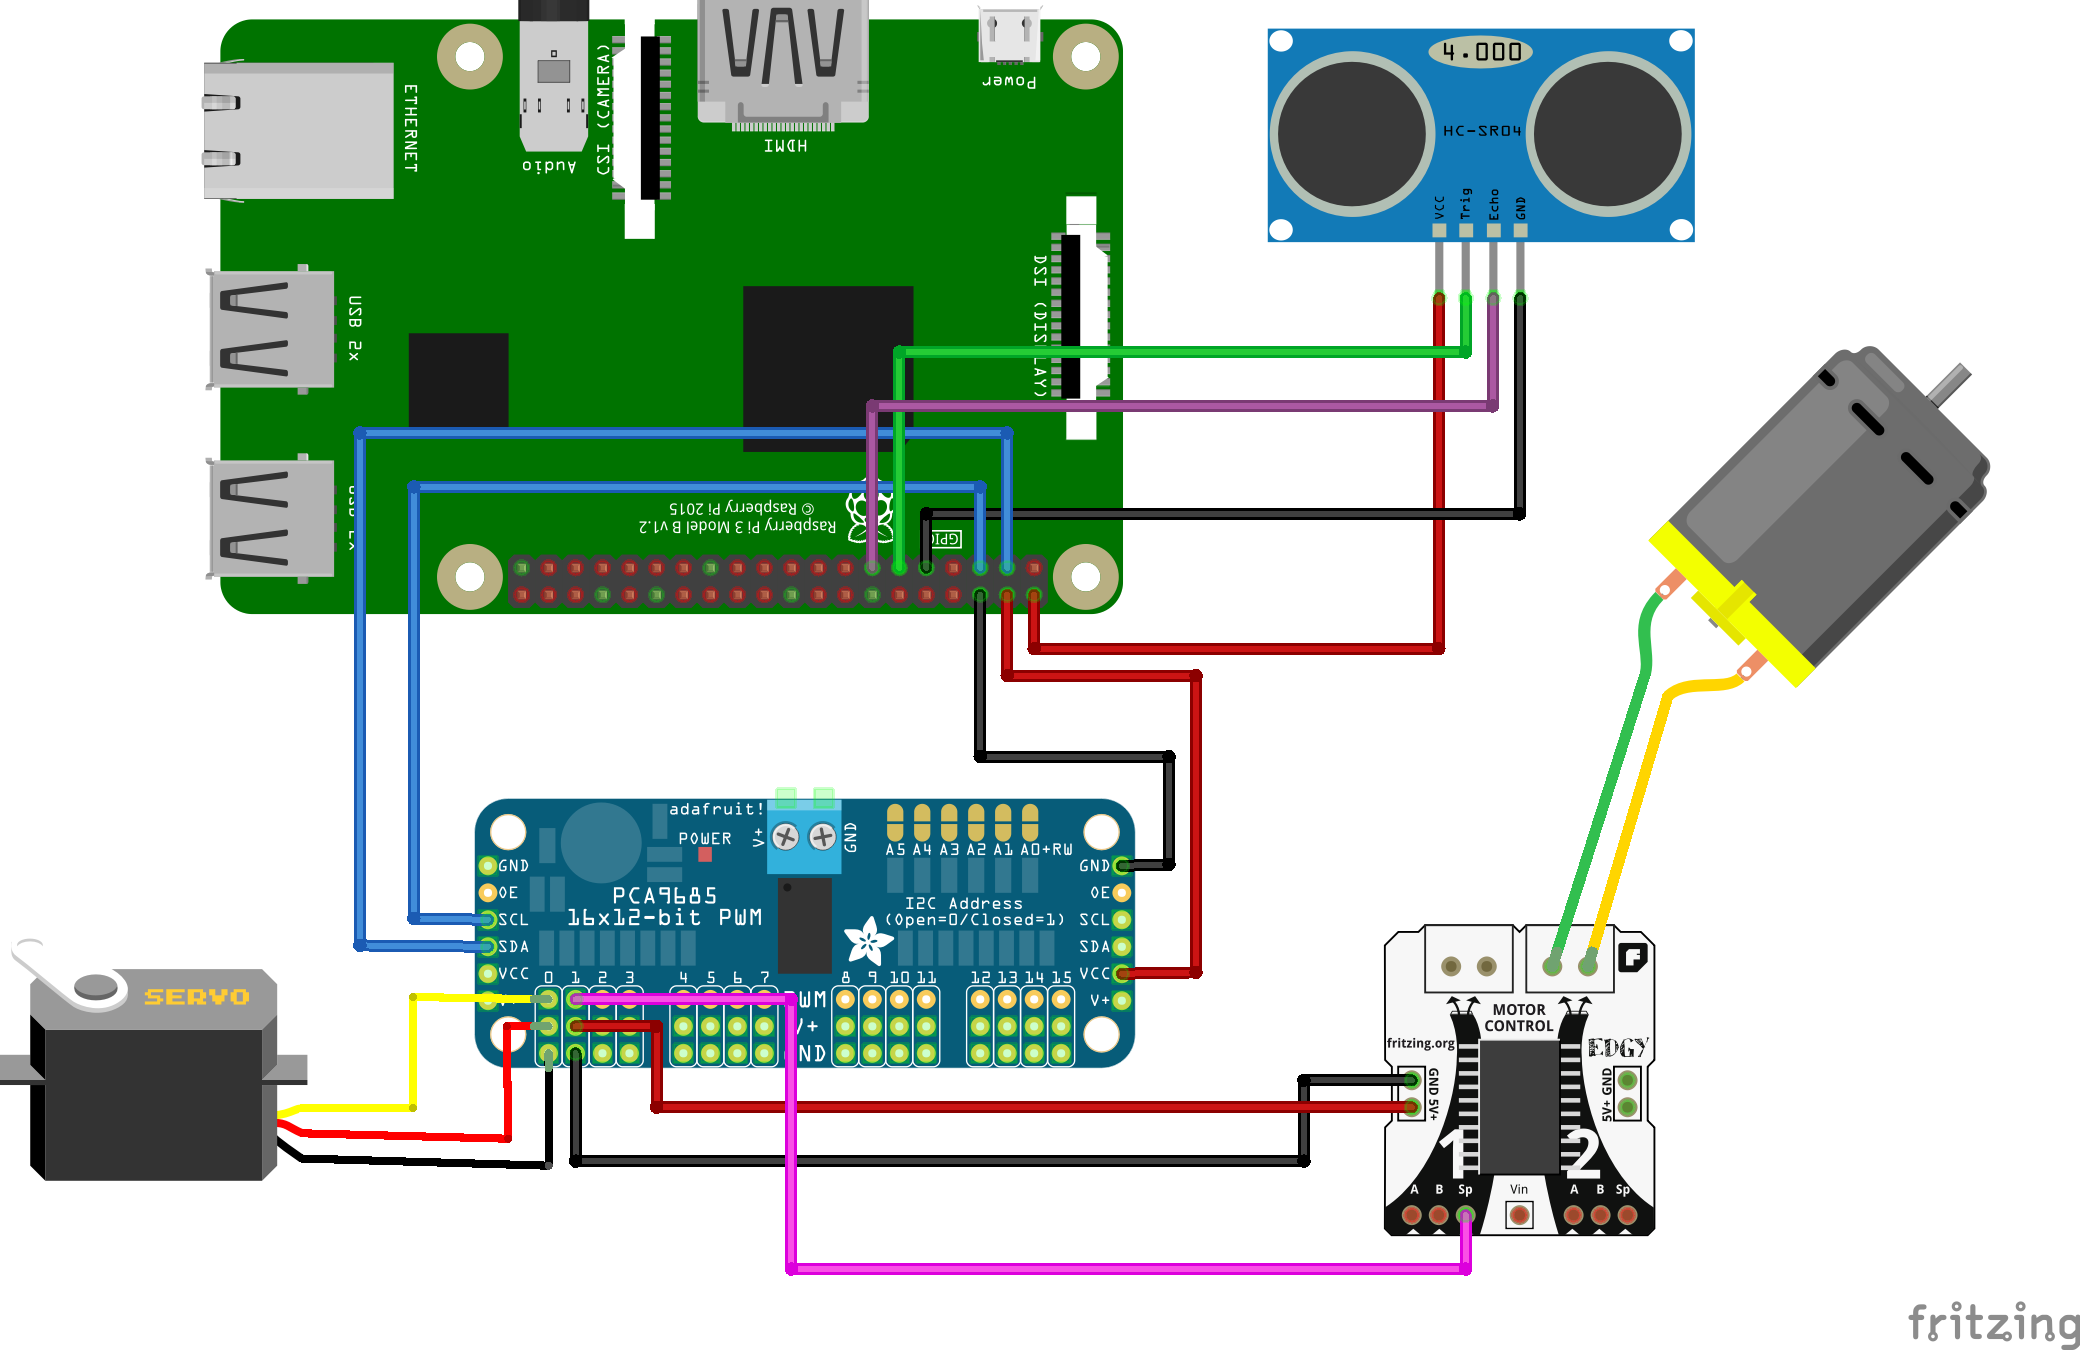
\includegraphics[width=1\linewidth]{images/hw_schematics.png}
      \caption{Beschaltung der Module}
      \label{fig:img-hw-06}
    \end{minipage}
    \vspace{1cm}

    \noindent
    Statt des EDGY Motor Control Moduls kommt in diesem Projekt der im RC
    Fahrzeug enthaltene Reely Fahrtenregler zum Einsatz. Die Anschlussbelegung
    ist weitesgehend dieselbe. \\

    \begin{minipage}{\columnwidth}
      \makeatletter
      \def\@captype{table}
      \makeatother
      \centering
      %\rowcolors{1}{grey}{white}
      \begin{tabular}{l | l | l | l}
      % \multicolumn{2}{|c}{Frame \#} & \multicolumn{4}{|c}{LCD 0/3} &
      GPIO Raspberry Pi & Modul & Pin & Beschreibung \\ \hline \hline
      2 / 5V & SR-04 & VCC & Spannungsversorgung \\
      3 / GPIO 2 & PCA9685 & SDA & I2C Datenleitung PWM Modul \\
      4 / 5V & PCA9685 & VCC & Spannungsversorgung PWM Modul \\
      5 / GPIO 3 & PCA9685 & SCL & I2C Taktsignal PWM Modul \\
      6 / GND & PCA9685 & GND & Masse PWM Modul \\
      9 / GND & SR-04 & GND & Masse Ultraschallsensor \\
      11 / GPIO 17 & SR-04 & TRIG & Trigger Impuls \\
      13 / GPIO 27 & SR-04 & TRIG & Echo \\
      
      \end{tabular}
      \caption{Pinbelegung}
      \label{tab:hw-01}
    \end{minipage}


  
  \section{Software}
    \ \\
    \subsection{Aufbau}
    \ \\
    \begin{minipage}{\columnwidth}
      \makeatletter
      \def\@captype{figure}
      \makeatother
      \centering
      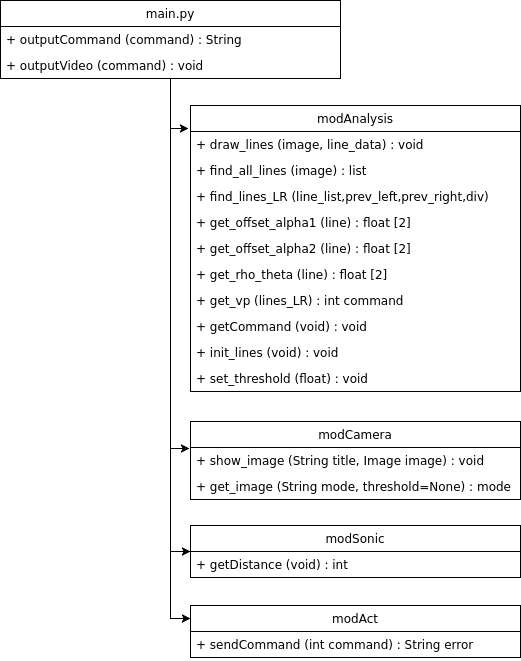
\includegraphics[width=0.8\linewidth]{images/code-flowchart.png}
      \caption{Aufbau des Python Codes}
      \label{fig:image-01}
    \end{minipage}
    \ \\

    \subsection{Externe Module}
    \ \\
    \begin{minipage}{\columnwidth}
      \makeatletter
      \def\@captype{table}
      \makeatother
      \centering
      %\rowcolors{1}{grey}{white}
      \begin{tabular}{ l | l }
      % \multicolumn{2}{|c}{Frame \#} & \multicolumn{4}{|c}{LCD 0/3} &
      Name & Beschreibung \\ \hline \hline
      tkinter & ... \\
      Adafruit\_PCA9685 & Bibliothek zur Ansteuerung des Motorcontrollers \\
      numpy & Bibliothek zur Verwendung von Matlab Funktionen \\
      cv2 & OpenCV 2 bietet Algorithmen zur Bildverarbeitung \\
      io & ... \\
      time & ... \\
      importlib & ... \\
      argparse & ... \\
      pivideostream & ... \\
      picamera & ... \\
      threading & ... \\
      RPi.GPIO & Bibliothek zur Ansteuerung der GPIO ports des Raspbery Pi \\
      \end{tabular}
      \caption{verwendete externe Python Module}
      \label{tab:01}
    \end{minipage}
    
    \subsection{Eigene Module}
    \ \\
    \begin{minipage}{\columnwidth}
      \makeatletter
      \def\@captype{table}
      \makeatother
      \centering
      %\rowcolors{1}{grey}{white}
      \begin{tabular}{ l | l }
      % \multicolumn{2}{|c}{Frame \#} & \multicolumn{4}{|c}{LCD 0/3} &
      Name & Beschreibung \\ \hline \hline
      modAnalysis & Verantwortlich für die eigentliche Verarbeitung der visuellen Informationen \\
      modAct & Verantwortlich für die Ansteuerung des Motors und der Lenkung \\
      modCamera & Bereitet das Kamerabild für die Verarbeitung und Anzeige vor. \\
      modSonic & Kommuniziert mit dem Ultraschallsensor und liefert Distanz zum Hindernis.\\
      \end{tabular}
      \caption{verwendete eigene Python Module}
      \label{tab:01}
    \end{minipage}



  \subsection{Funktionen aus der openCV Library}
OpenCV ist eine open-source Bibliothek mit Algorithmen für die 
  Bildverarbeitung und maschinelles Sehen (siehe auch opencv.org)Sie. Sie ist u.a. für die
Programmiersprache Python geschrieben und beinhaltet Funktionen, die für die
Fahrbahnlinienerkennung eingesetzt werden.\\
\subsubsection{Canny-Edges Filter}

\begin{minipage}{\columnwidth}
  \makeatletter
  \def\@captype{figure}
  \makeatother
  \centering
  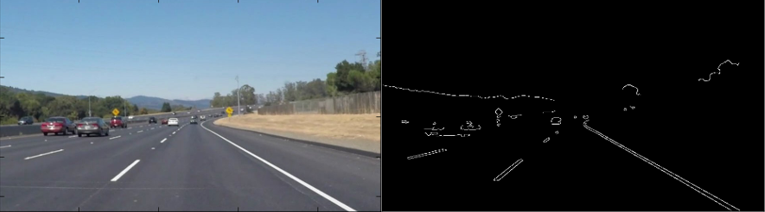
\includegraphics[width = 0.8\linewidth]{images/cannyEdgesExample.png}
  \caption{Beispiel: Fahrbahnbild und Canny-Edges-Filter}
  \label{fig:cannyExample}
\end{minipage}{
\vspace{0.8cm}
  
Der Canny-Edges-Filter wird im Kamera-Modul angewendet und über
\begin{lstlisting}
openCV.Canny("image-file", int lowerTreshold, int upperTreshold)
\end{lstlisting}
aufgerufen. Die Funktion liefert ein binäres Bild, das die Umrisse
  von Bildobjekten in weiß auf schwarzem Hintergrund darstellt
(siehe Abb.\ref{fig:cannyExample}).\\
Nach einem Rauschfilter, der im Hintergrund läuft, wird der Gradient
für jedes Pixel bestimmt. Liegt ein Gradient unterhalb des
\textit{untererThresholds},
wird ein Pixel schwarz im Zielbild, ist der Gradient oberhalb des
\textit{upperThresholds}, wird ein weißes Pixel ins Zielbild geschrieben. 
Gradientwerte im Zwischenbereich werden als schwarz geschrieben, es sei denn, 
sie sind mit Gradienten im Bild verbunden, die oberhalb des Thresholds liegen.\\
Die Einstellungen des Thresholds sind ein sensibler Bereich, da hier eine
Voretnscheidung getroffen wird, welche Bildinformationen erhalten bleiben bzw.
verworfen werden. Idealerweise würden hier nur die Umrisse der Fahrbanlinien
ausgewählt werden.\\

\subsubsection{Hough-Transformation}

\begin{minipage}{\columnwidth}
  \makeatletter
  \def\@captype{figure}
  \makeatother
  \centering
  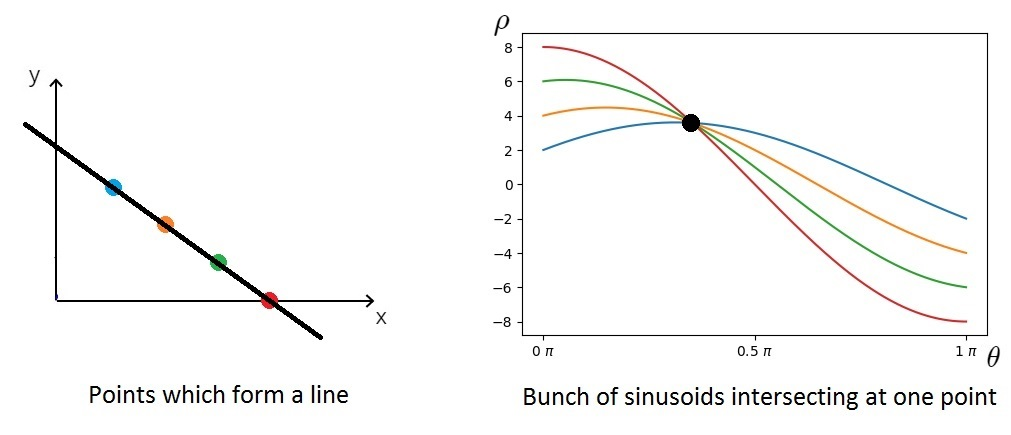
\includegraphics[width = 0.8\linewidth]{images/exampleHough.jpg}
  \caption{Beispiel: Darstellung einer Geraden kartesisch und im Hough-Raum}
  \label{fig:cannyExample}
\end{minipage}
\vspace{0.8cm}

Die Houghtransformation wird mit opencv.HoughLines(image, rho, theta, threshold) aufgerufen und gibt einen
Vektor zurück mit allen im Bild erkannten Lininen, die jeweils mit dem
Wertepaar($\rho$, $\theta$) beschrieben werden.Für $\rho$ und $\theta$ wird durch den Wert
ein Toleranzwert beschrieben. "threshold" bezeichnet einen Wert, der
die Mindestanzahl von Punkten bestimmt, die vorliegen müssen, damit eine Grade
als beschrieben gilt.\\
Die Funktion wird zweimal angewendet: zum Einen beim Start zur Initialisierung,
daß im gegeben Kamerabild die Fahrbahnlinien erkannt werden. Hierbei wird mit
einem größeren Toleranzbereich gearbeitet, um eine Erkennung sicherzustellen.
Zum anderen wird für jedes Bild des Kamerastreams die Linienerkennung gemacht,
und mit einem strengeren Toleranzbereich mit den aus dem Vorbild erkannten
Linienpaar verglichen. Dadurch soll verhindert werden, dass weitere erkannte
Linien, die nicht Teil der Fahrbahn sind, fehlerhaft in die erkannten Linien mit
einbezogen werden.\\
Die so noch erkannten Linien werden anhand von rho nd theta  entweder der linken 
oder der rechten Fahrbahnlinie zugeordnet, und für beide Seite eine Linie
gemittelt und als neue Orientierungslinen zur Richtungsbestimmung genutzt.\\
  
  
  \section{Werkzeuge der Bildverabreitung}
Die folgende Zusammenfassung der Thematik basiert auf dem Buch
"Digitale Bildverarbeitung" von Burger, Burge \citep{BurgeDigitBild}, das als 
Standartliteratur zu empfehlen ist. Eine zusammenfassende Wiedergabe der für 
das Projekt relevanter Themen ist im Folgenden nachzulesen.\\
Ein Bestandteil der Bildverarbeitung ist die Bildanalyse, bei der
sinnvolle Informationen aus Bildern extrahiert werden. Genauer ist der Themenbereich
\textit{Computer Vision} gemeint, bei dem es um das Mechanisieren von
Sehvorgängen des Menschen in der dreidimensionalen Welt geht.\\
Die Steuerung des Wagens soll durch Informationen aus den Kamerabildern
erfolgen: Durch Erkennen der Fahrbahnlinien wird der Lenkungsservo geregelt, der
das Auto innerhalb der Spur zwischen den Fahrpahnlinien hält.\\
Dieser Prozess lässt sich in Einzelschritten beschreiben mit:
\begin{enumerate}
  \item \textit{Digitalisierung} der dreidimensionalen Welt mit Hilfe der Kamera
  \item \textit{Vorverarbeitung} (Bildverbesserung bzw. Anpassung an den Zweck) durch
    Umwandlung in ein binäres Canny-Edges-Bild
  \item \textit{Segmentierung} durch Vorauswahl des Bildauschnittes mit den relevante
    Informationen
  \item \textit{Merkmalsextraktion} zur Linienerkennung durch die Hough-Transformation
  \item \textit{Parametrisierung} als mathematische  Beschreibung der Fahrbahnlinien zur
    weiteren Informationsverarbeitung
\end{enumerate}

\subsection{Digitalisierung}
Der von der Kamera aufgenommen Bilder-Stream liegt in digitaler Form vor. Dabei lassen
sich benötigte Parameter eintellen. Um ein optimales Bild zu
erhalten sind die Beleuchtungsumstände zu beachten, da hierdurch die
Differenzierung von Linien im Bild erheblich beeinflusst wird.\\
Anzumerken ist hier, dass in der Bildverabreitung der Ursprung des
Koordinatensystems bzw. der x- und y-Achse in der linken
oberen Ecke des Bildes definiert ist.

\subsection{Vorverarbeitung - Der Canny-Kantenoperator}
Zur späteren Erkennung der Linien werden die dafür relevanten Informationen aus
dem Bild gefiltert: sogenannte Bildkannten. Bildkanten sind Übergangsstellen, wo
ein hoher Grauwertsprung von einem Pixel zum Nachbarpixel vorliegt, wie z. B. bei 
einem weißen Farbahnstreifen auf dunkler Fahrbahn, hier werden zwei Kannten
analysiert. Kanten werden dem entsprechend an diversen Stellen im Bild
detektiert, deshalb sind die Parameter entsprechend zu wählen.\\
Die Canny-Edges-Funktion ist ein bewährter Algorithmus zur Kantenerkennung, da drei Ziel
gleichzeitig erreicht werden drei Ziele: ein zuverlässiges Detektieren
vorhandener Kanten, die Position der Kante präzise zu bestimmen, und Farbsprünge, 
die nicht als Kante interoretiert werden sollen, auszulassen. Diese Funktion
ist in der OpenCV-Library enthalten. \\

\subsection{Segmentierung}
[BILD Kamera mit Fahrbahnlinien]
Der für die Erkennung der Fahrbahnlinien relevante Bereich liegt in einem
unteren Dreieck des Kamerabildes. Dieser Teil wird ausgewählt, bzw. davon ausserhalb
liegende Bereiche werden nicht bei der Erkennenung der Farbahnlinien
berücksichtigt.\\

\subsection{Merkmalsextraktion zur Linienerkennung}
Das Canny-Kantenbild wird mit Hilfe der Hough-Transformation aus der
openCV-Library in den Hough-Raum transformiert, wo dann die Erkennung der Linien
erfolgt.

\begin{minipage}{\columnwidth}
  \makeatletter
  \def\@captype{figure}
  \makeatother
  \centering
  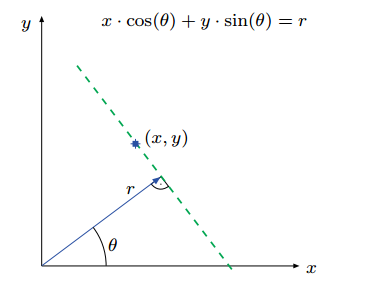
\includegraphics[width=0.8\linewidth]{images/gradeThetaR.png}
  \caption{Beschreibung einer Graden durch Winkel und Abstand vom Ursprung}
  \label{fig:gradeThetaR}
\end{minipage}

Dabei kommt zur Anwendung, dass eine Gerade mathematisch sowohl mit $y
= m \cdot x + b$ als auch mit $r(\theta) = x \cdot cos(\theta) + y \cdot
sin(\theta)$ beschrieben werden kann. Dabei ist in der zweiten Beschreibung 
$\theta$ der  Winkel des Radius $r$ zum Urspung, an dessen Ende senkrecht die
beschriebene Grade verläuft. Zu Bedenken ist, dass wie schon erwähnt der
Koordinatenursprung des Bildes oben links definiert ist.\\
Das rechenaufwendige Verfahren der Hough-Transformation generiert für jeden
Kantenbildpunkt des Canny-Edges-Bildes Bildpunkte im Hough-Raum, dessen Achsen
ein $\theta$ / $r$ - Koordinatensystem bilden. Linien im kartesisches System
sind als Punkthäufungen im Hough-Raum erkennbar. Liegt eine Anzahl von
Punkten oberhalb eines zu definierenden Schwellwertes, wird eine Linie erkannt
und die Houh-Transformationsfunktion gibt ein Wertpaar $\theta$, $r$ zurück.
 
  
  \section{Iterative Auswertung des Kamerabildes}	

	Das Bild der Kamera werden iterativ ausgewertet um die beiden Fahrbahnlinien zu erkennen und daraus ein Ausgangssignal für die Steuerung zu generieren. Der gewählte Ansatz war es, die Fahrbahnlinien durch zwei Geraden anzunähern. Die Funktion HoughLines wird verwendet um die Fahrbahnlinien zu erkennen und die zugehörigen Geraden zu berechnen. Da die Funktion HoughLines in den meisten Fällen nicht nur die beiden Fahrbahnlinien erkennt, sondern alle möglichen Geraden, bestand die erste Aufgabe darin, nur die Geraden herauszufiltern, welche die Fahrbahnlinien repräsentieren, und alle anderen Geraden zu verwerfen. Im Programm wird dies erreicht, indem alle Geraden, die durch die Funktion HoughLines gefunden wurden mit dem Geradenpaar aus dem vorherigen Programmdurchlauf verglichen werden, und nur ähnliche Geraden beibehalten werden.\\
	
	Beim Start des Programm werden für die beiden Geraden feste Werte vorgegeben, die dann korrigiert und an die erkannten Fahrbahnlinien angepasst werden. In Abbildung \ref{fig:fahrbahn} ist dies bildlich dargestellt. Die roten Linien sind zu Beginn des Programms fest vorgegeben. Die blauen Linien sind das Ergebnis der Korrektur durch das Programm.
	
	\begin{figure}[H]
		\centering
		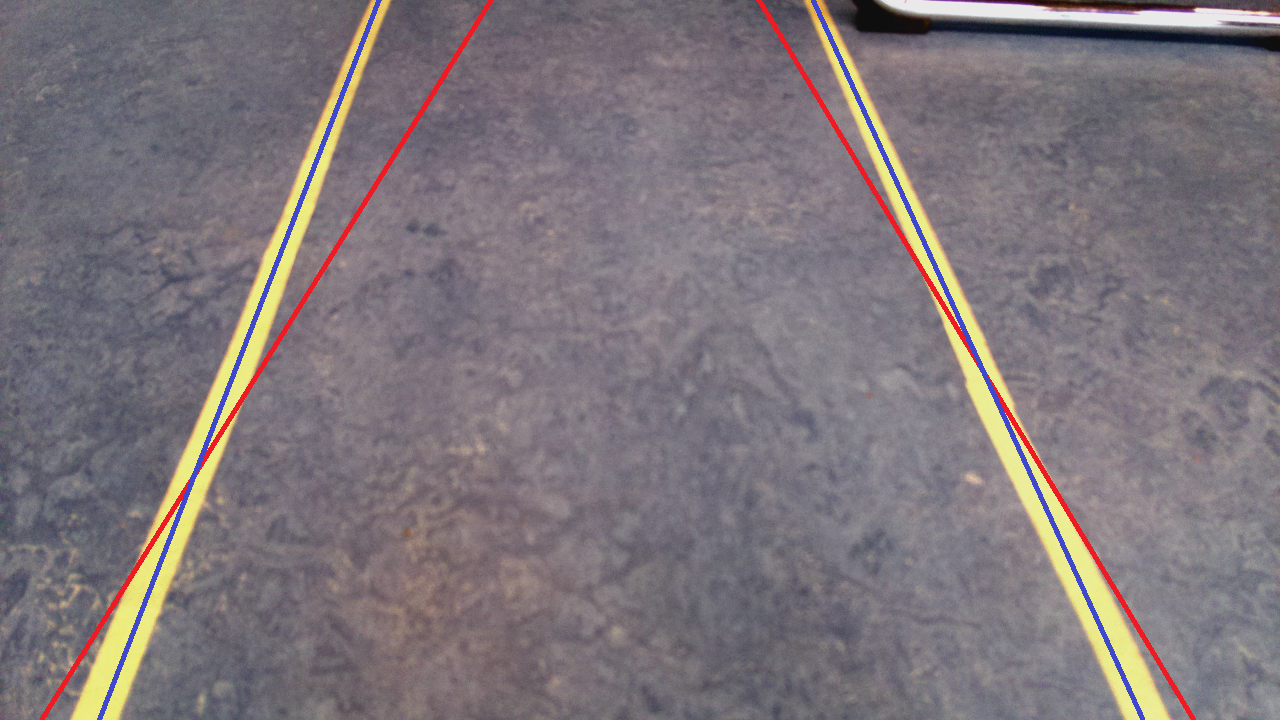
\includegraphics[width=.5\linewidth]{images/fahrbahn.png}
		\caption{Korrektur der vorgegeben Geraden}
		\label{fig:fahrbahn}
	\end{figure}
	
	
	Der Vergleich der Geraden wird durchgeführt, indem um die beiden Geraden aus dem letzten Durchlauf ein Toleranz-Fenster gelegt wird, und von allen gefundenen Geraden nur diejenigen herausgefiltert werden, die innerhalb dieses Toleranz-Fensters liegen. Von diesen Geraden wird dann der Durschnitt berechnet, sodass nur noch zwei Geraden für die beiden Fahrbahnlinien übrig bleiben. \\
	
	Eine Schwierigkeit besteht darin die Geraden so zu repräsentieren, dass diese gut miteinander vergleichbar sind. Bei einer geringen Änderung einer Geraden von einem zum nächsten Zyklus sollen sich deren Parameter dabei auch nur geringfügig ändern. Ansonsten werden ähnliche Geraden beim filtern verworfen, da deren Parameter nicht im Toleranzfenster liegen. Im Programm wurden daher je nach Anwendungsfall verschiedene Repräsentationsformen verwendet, welche im folgenden beschrieben werden.
	
	\subsection{Verwendete Repräsentationsformen von Geraden}
	
	Die Funktion HoughLines gibt als Ergebnis eine Liste von Geraden aus, die durch die beiden Parameter $\rho$ und $\theta$ beschrieben werden. $\theta$ ist der Winkel zwischen der Normalen, die senkrecht auf der Geraden steht, und der x-Achse. Der Winkel  $\rho$ ist die Länge dieser Normalen, d.h. der Abstand zwischen der Geraden und dem Ursprung des Koordinatensystems. Der Winkel $\theta$ ist immer positiv, $\rho$ kann, je nach Lage der Geraden positiv oder negativ sein.
	Abbildung \ref{fig:rho_theta1} zeigt ein Beispiel für die Repräsentation zweier Fahrbahnlinien durch einen Abstand $\rho$ und einen Winkel $\theta$, für den Fall, dass der Wagen relativ mittig und gerade auf der Fahrbahn steht. Dabei symbolisiert das Rechteck die Ränder des Kamerabildes, der Koordinatenursprung liegt in der oberen linken Ecke. $\theta_R$ und $\rho_R$ sind die Parameter der rechten Fahrbahnlinie, $\theta_L$ und $\rho_L$ die der Linken.
	
	\begin{figure}[H]
		\centering
		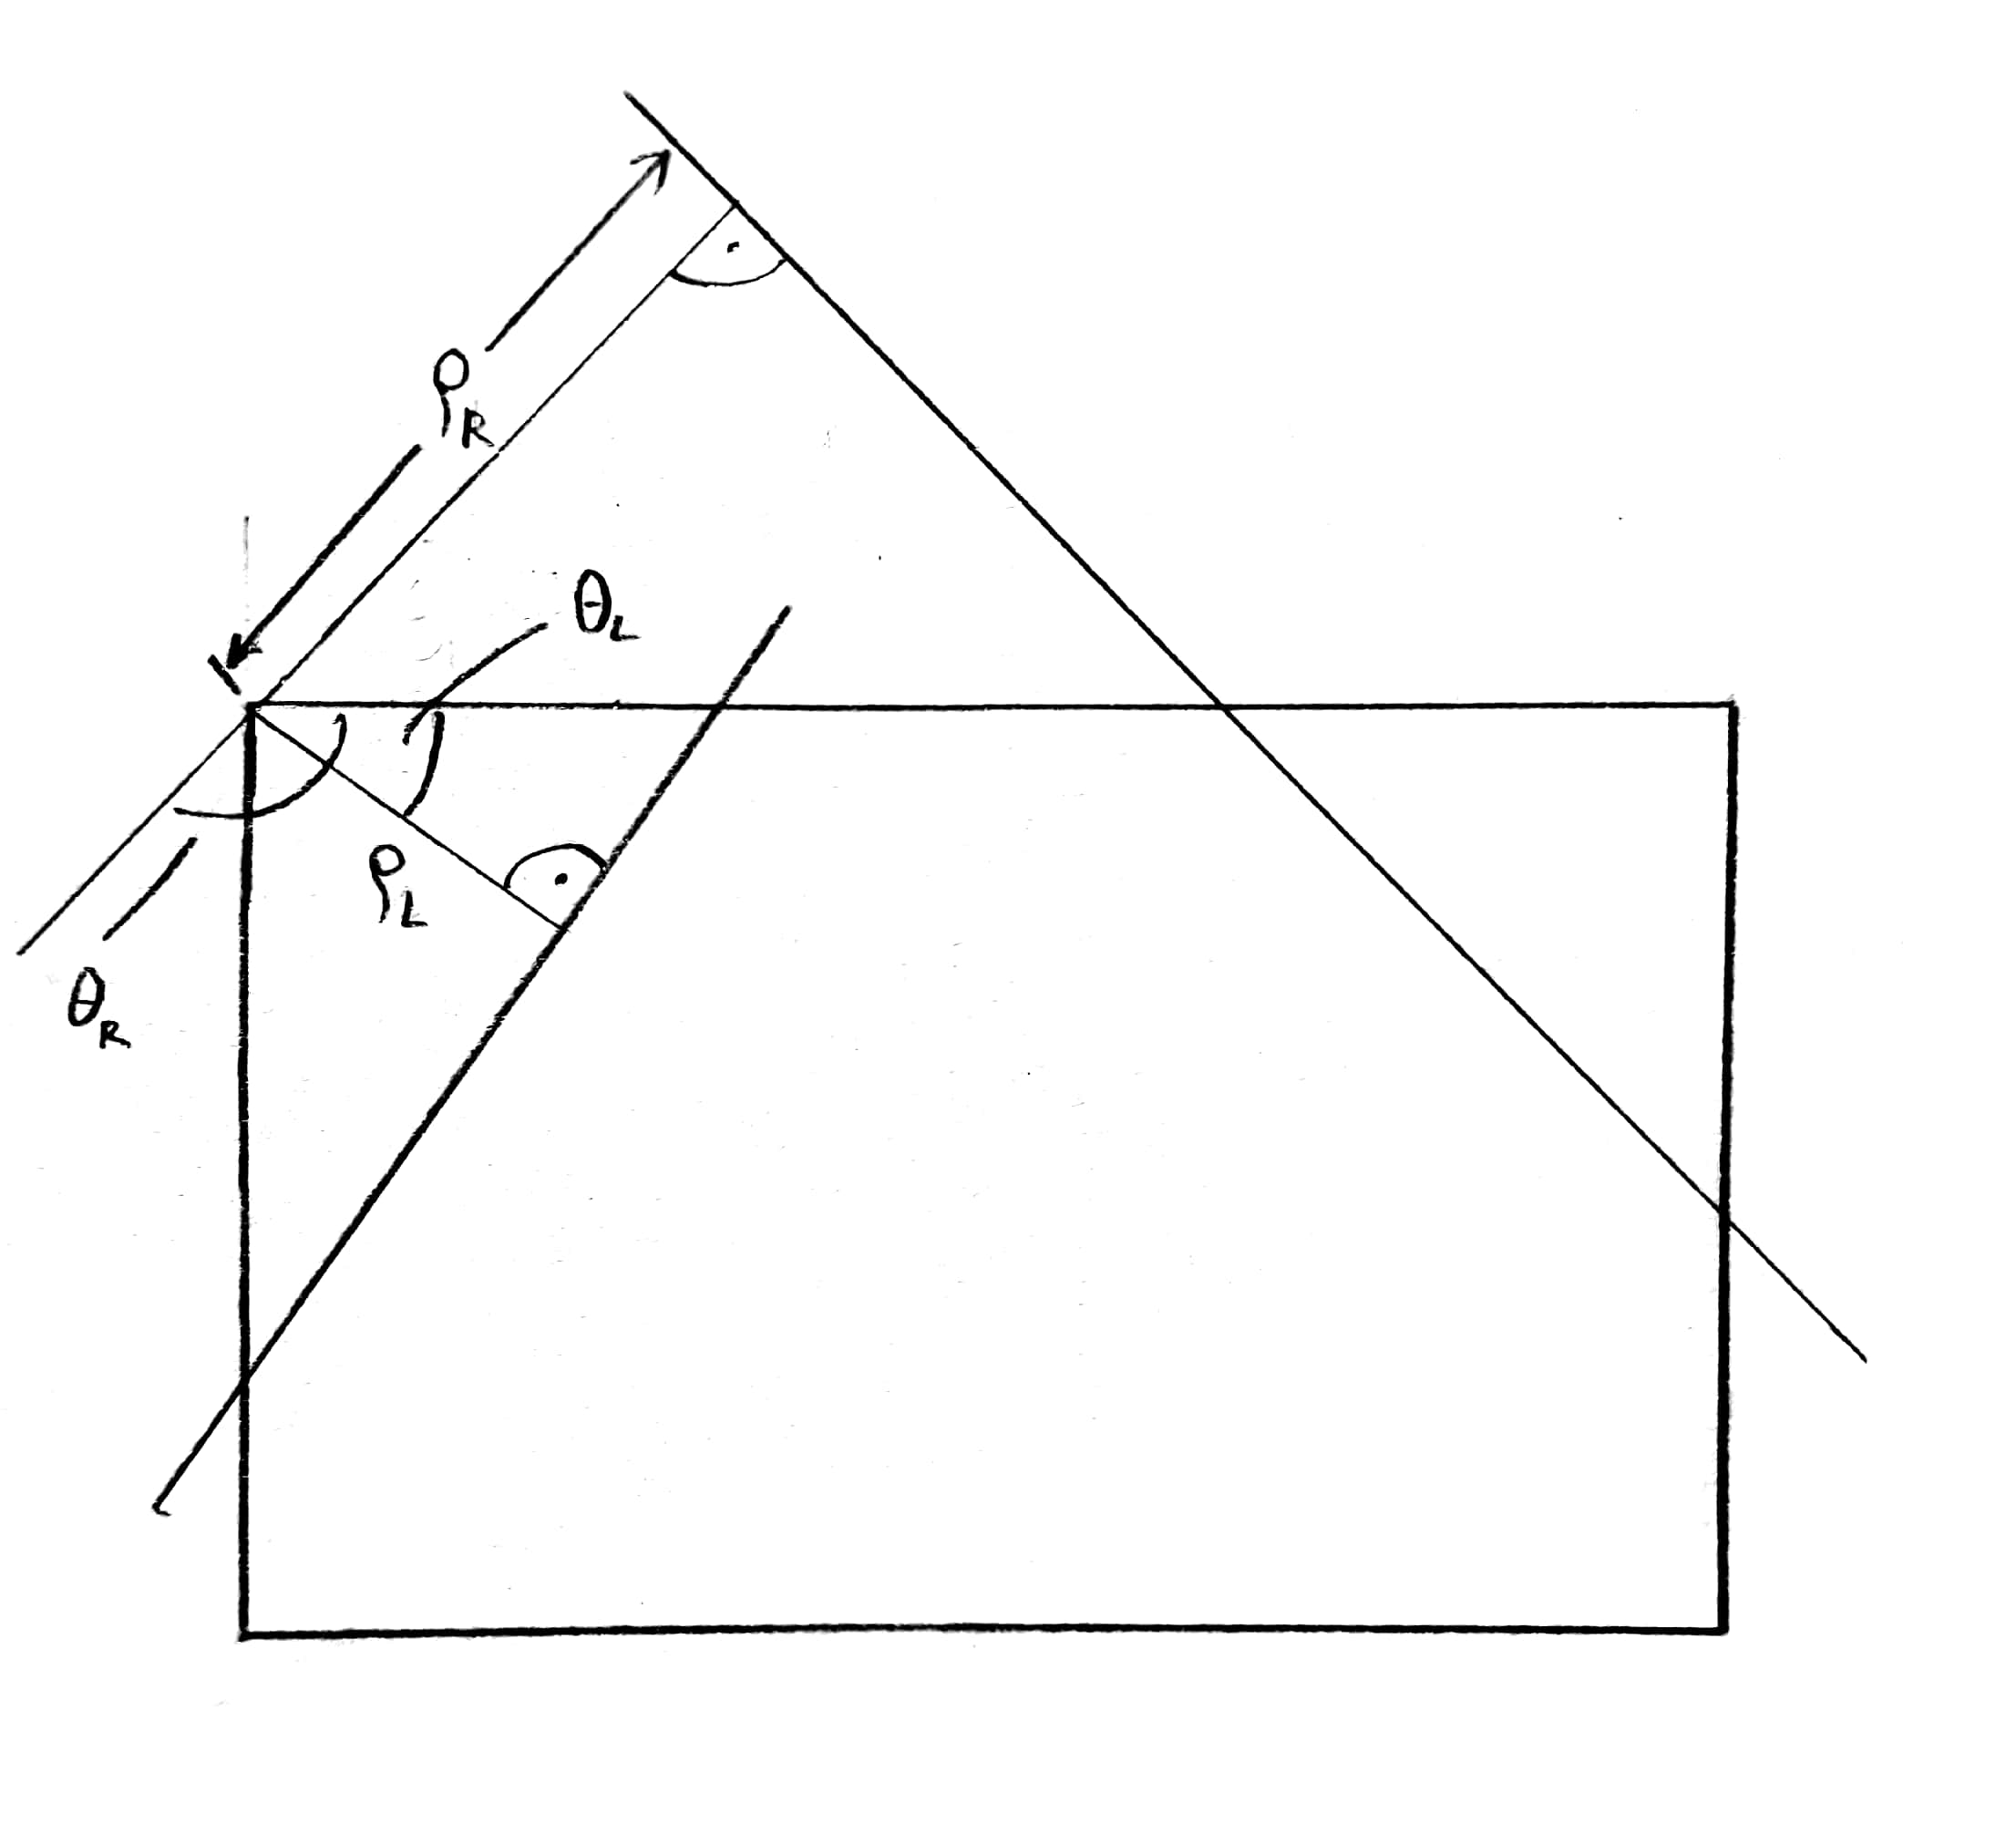
\includegraphics[width=.5\linewidth]{images/rho_theta1.jpg}
		\caption{Beispiel für die Geradenrepräsentation durch einen Winkel $\theta$ und einen Radius $\rho$}
		\label{fig:rho_theta1}
	\end{figure}
	
	Diese Form der Geradenrepräsentation ist jedoch problematisch, wenn es darum geht, zwei Geraden miteinander zu vergleichen. Ein Beispiel ist in Abbildung \ref{fig:rho_theta2} dargestellt. Hier beträgt die Änderung der Winkel $\theta_R$ und $\theta_L$ der beiden Fahrbahnlinien $\Delta\theta=5^\circ$, obwohl die Position der rechten Fahrbahnlinie sich viel mehr verändert hat, als die der linken.
	
	
	
	\begin{figure}[H]
		\centering
		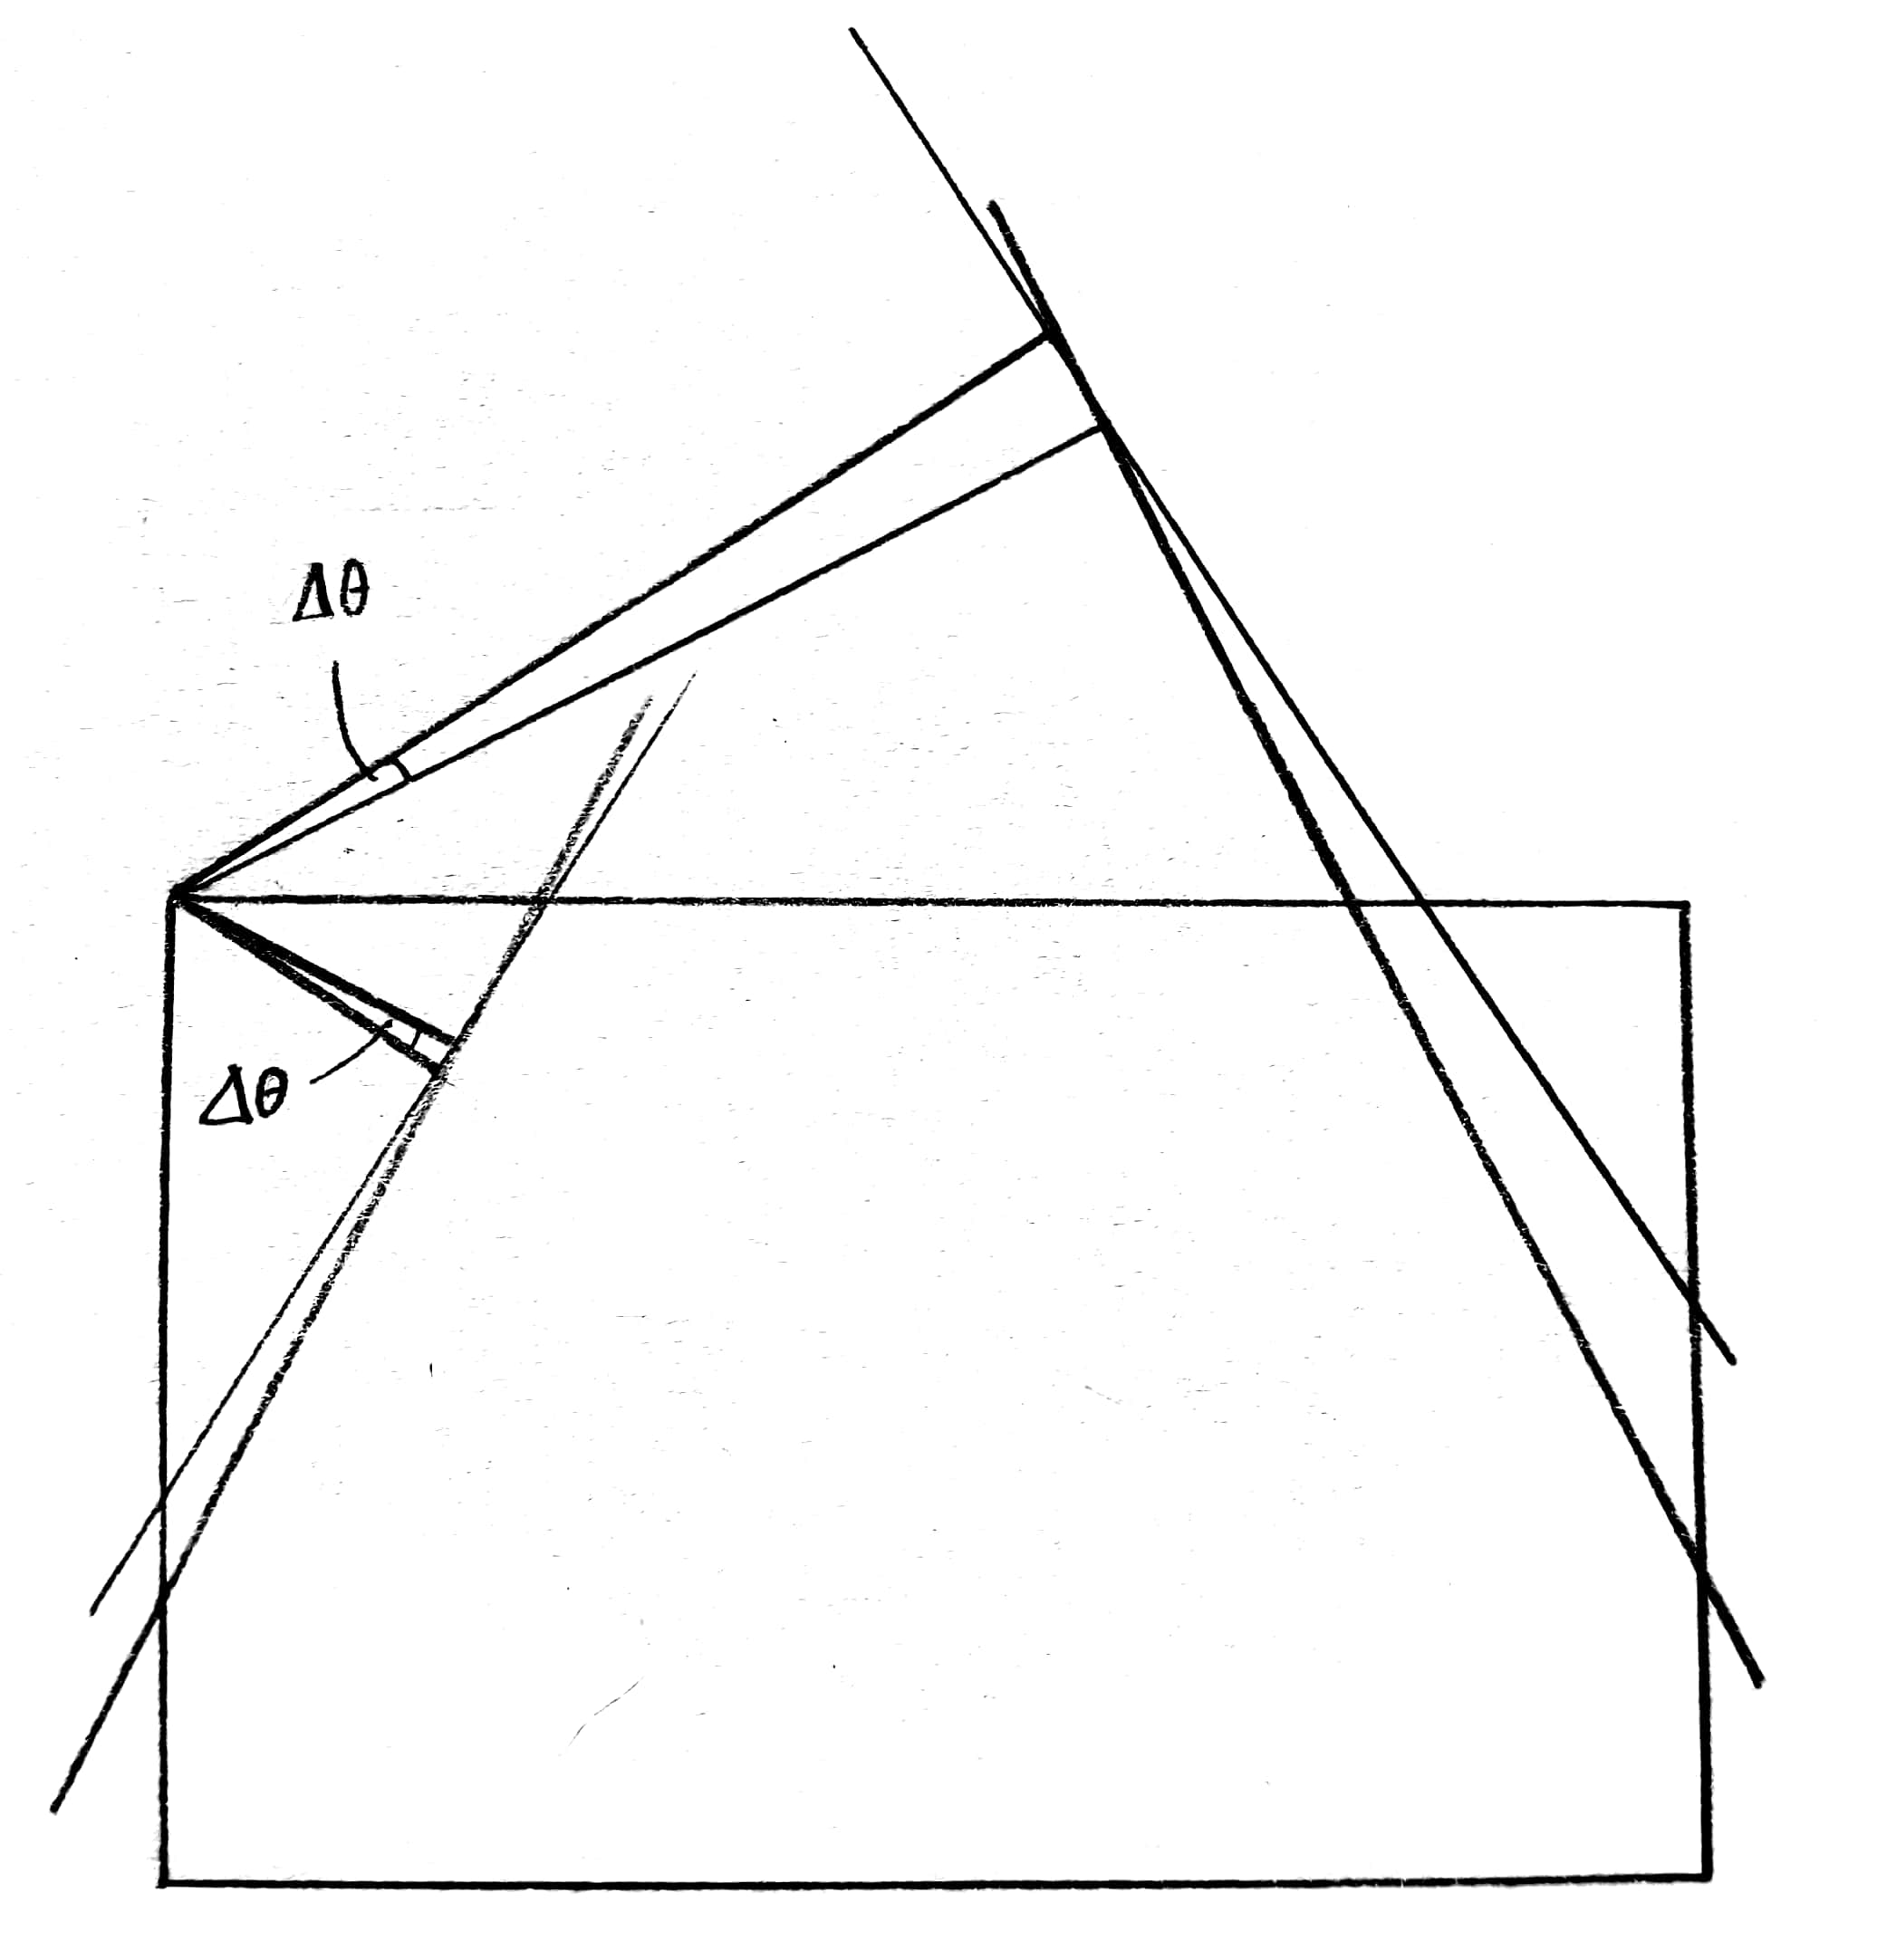
\includegraphics[width=.5\linewidth]{images/rho_theta2.jpg}
		\caption{Problematik bei dieser Form der Geradenrepräsentation}
		\label{fig:rho_theta2}
	\end{figure}

	Um dieses Problem zu beheben wurden die Geraden mithilfe der Funktion get\_offset\_alpha1 in eine andere Form umgerechnet, bei der diese durch den Offset $\omega$ auf der y-Achse und den Winkel zur x-Achse beschrieben werden. Die Umrechnung von der $\rho$-$\theta$-Form erfolgt folgendermaßen:\\

	
	
	Für Winkel $\theta<90^\circ$ (linke Fahrbahnlinie):
	
	\begin{align*}
	\alpha=90^{\circ}-\theta
	\omega&=-\frac{\rho}{\cos{90^{\circ}-\theta}} \\
	\end{align*}
	
	Für Winkel $\theta>90^\circ$ (rechte Fahrbahnlinie):
	
	\begin{align*}
	\alpha=\theta-90^{\circ}
	\omega&=-\frac{\rho}{\cos{\theta-90^{\circ}}} \\
	\end{align*}
	
	Abbildung \ref{fig:alpha_omega1} veranschaulicht die Repräsentation der beiden Fahrbahnlinien in dieser Form.
	
	\begin{figure}[H]
		\centering
		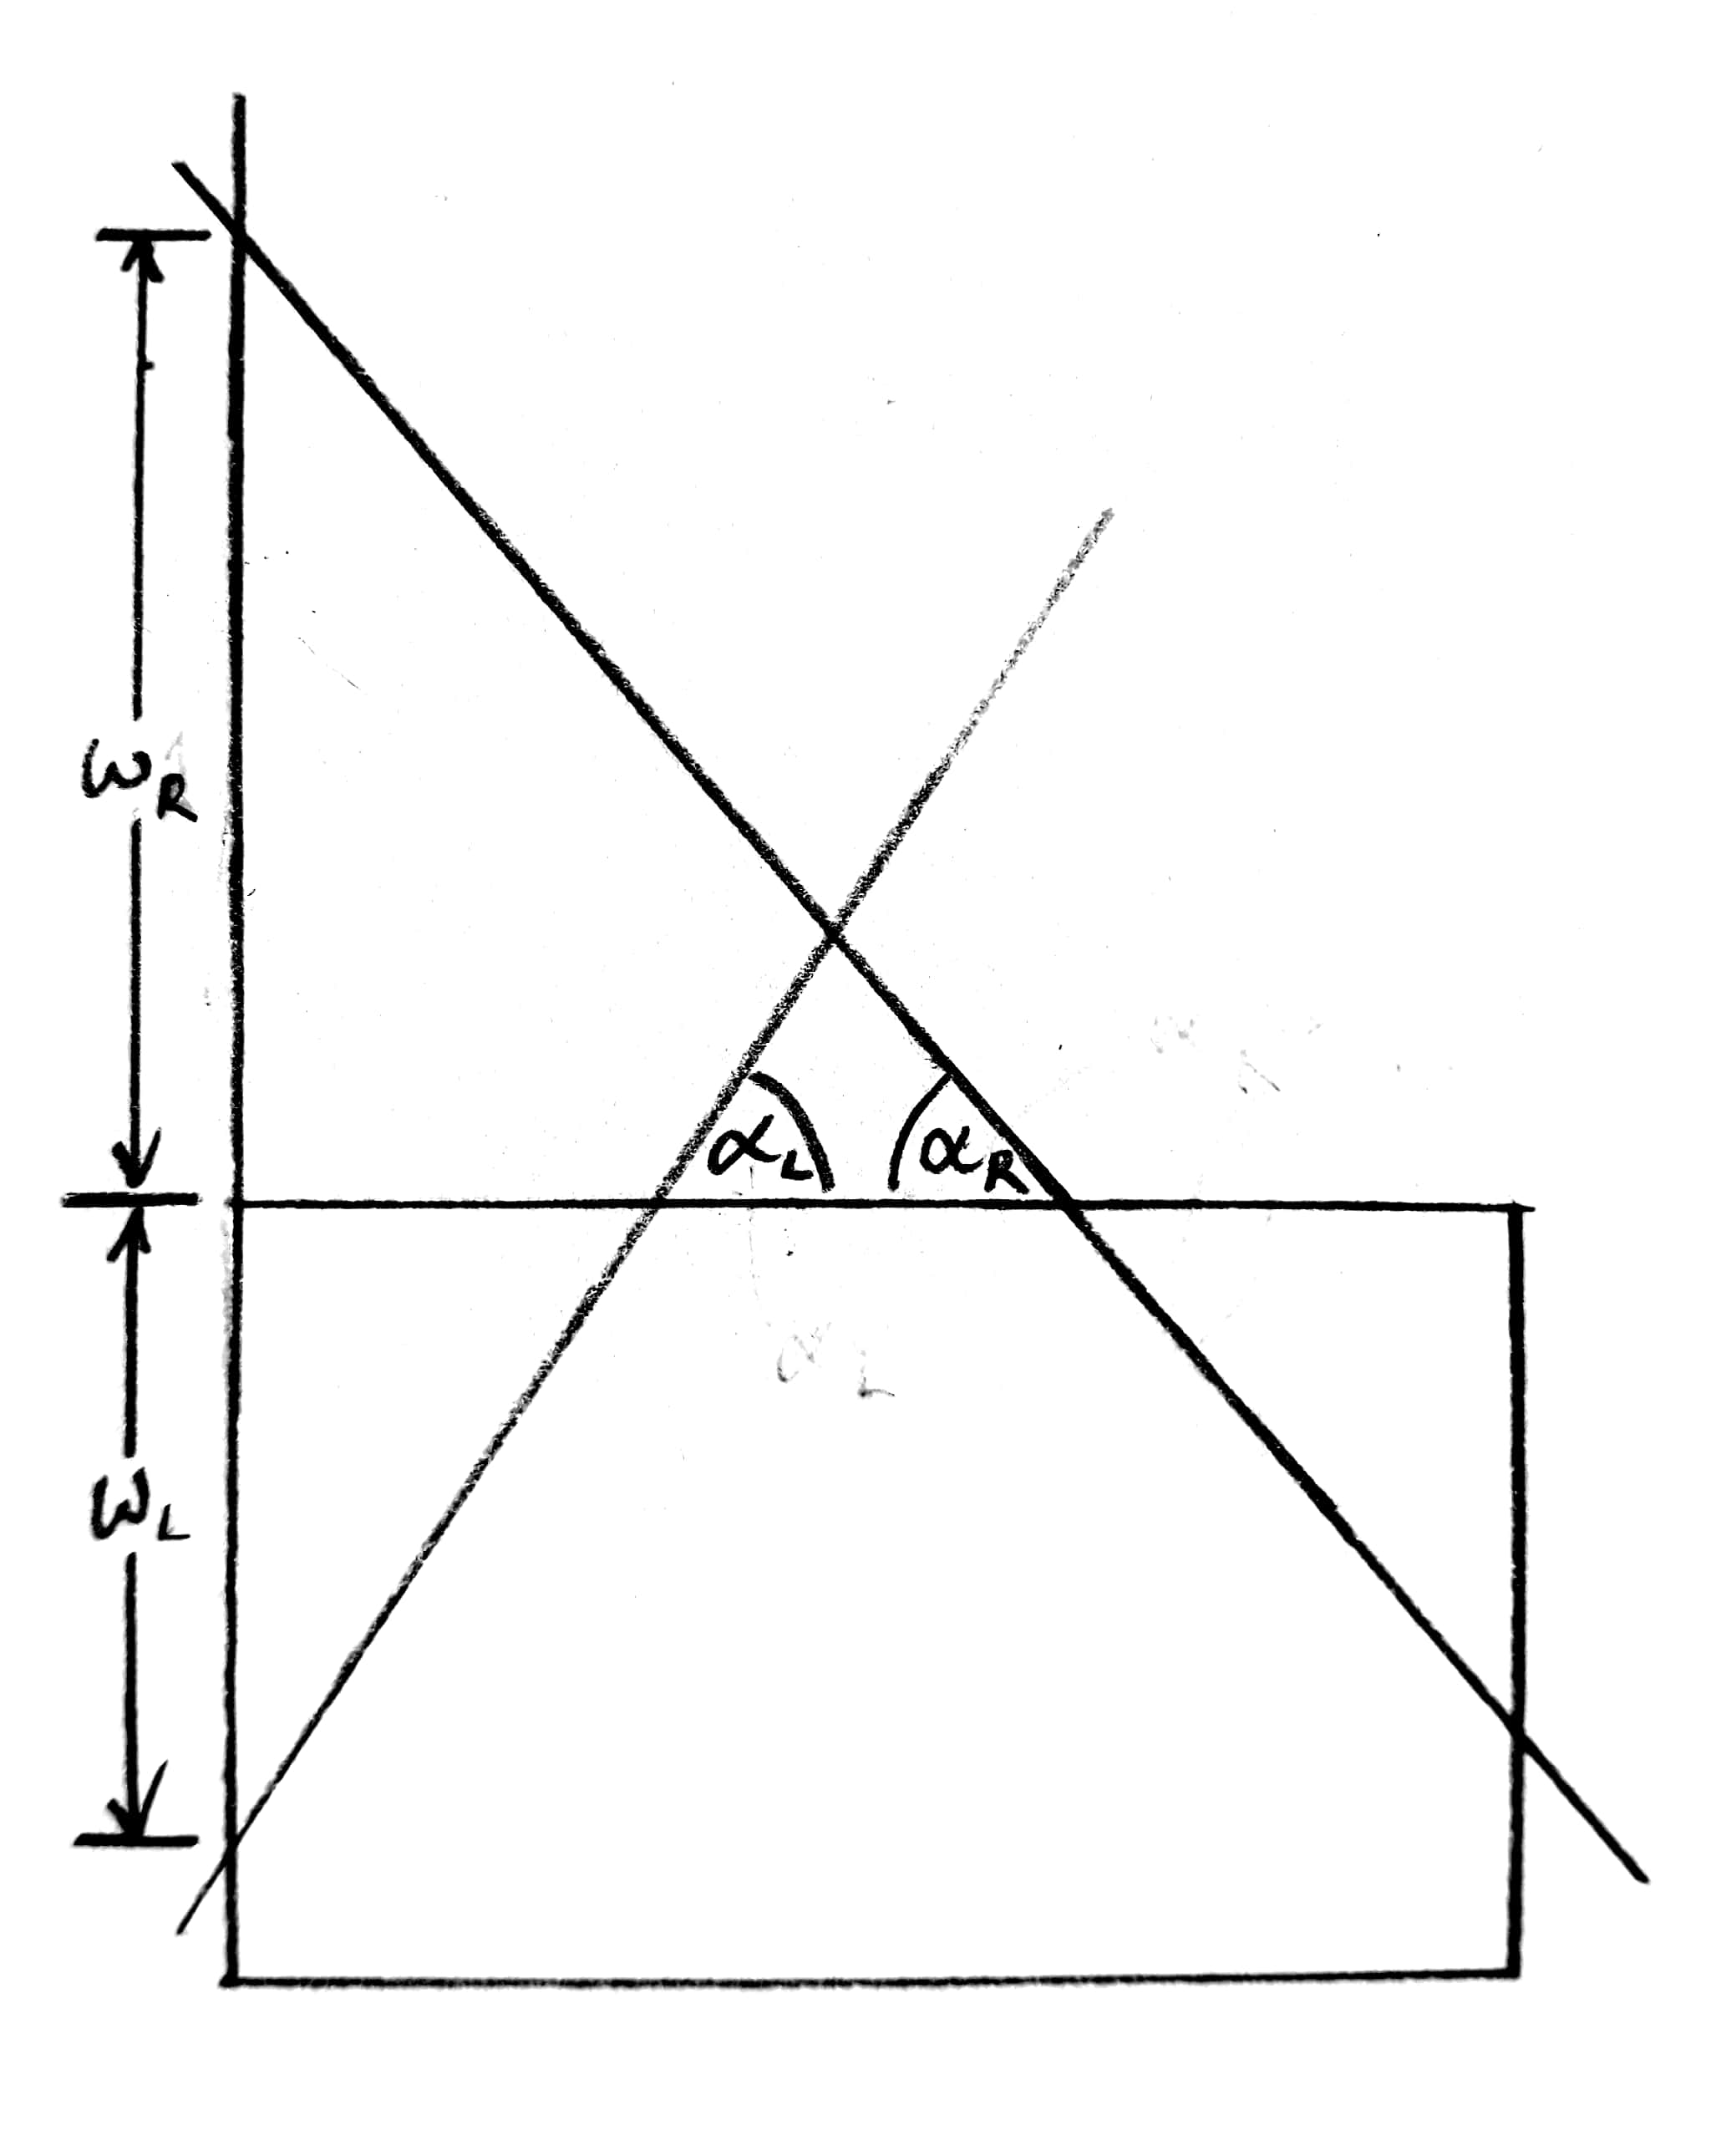
\includegraphics[width=.5\linewidth]{images/alpha_omega1.jpg}
		\caption{Beispiel für die Geradenrepräsentation durch einen Offset $\omega$ und einen Winkel $\alpha$}
		\label{fig:alpha_omega1}
	\end{figure}

	Bei dieser Form ergibt sich jedoch das Problem, dass sich bei steilen Geraden der Offset stark ändert, auch wenn der Winkel sich nur leicht ändert. Dadurch werden diese Geraden dann ungewollt verworfen. Dies ist besonders für die rechte Fahrbahnlinie der Fall, wie sich in Abbildung \ref{fig:alpha_omega2} erkennen lässt. Hier sieht man, dass sich der Offset $\omega$ stark ändert, auch wenn sich der Winkel der Geraden nur leicht ändert.


	\begin{figure}[H]
		\centering
		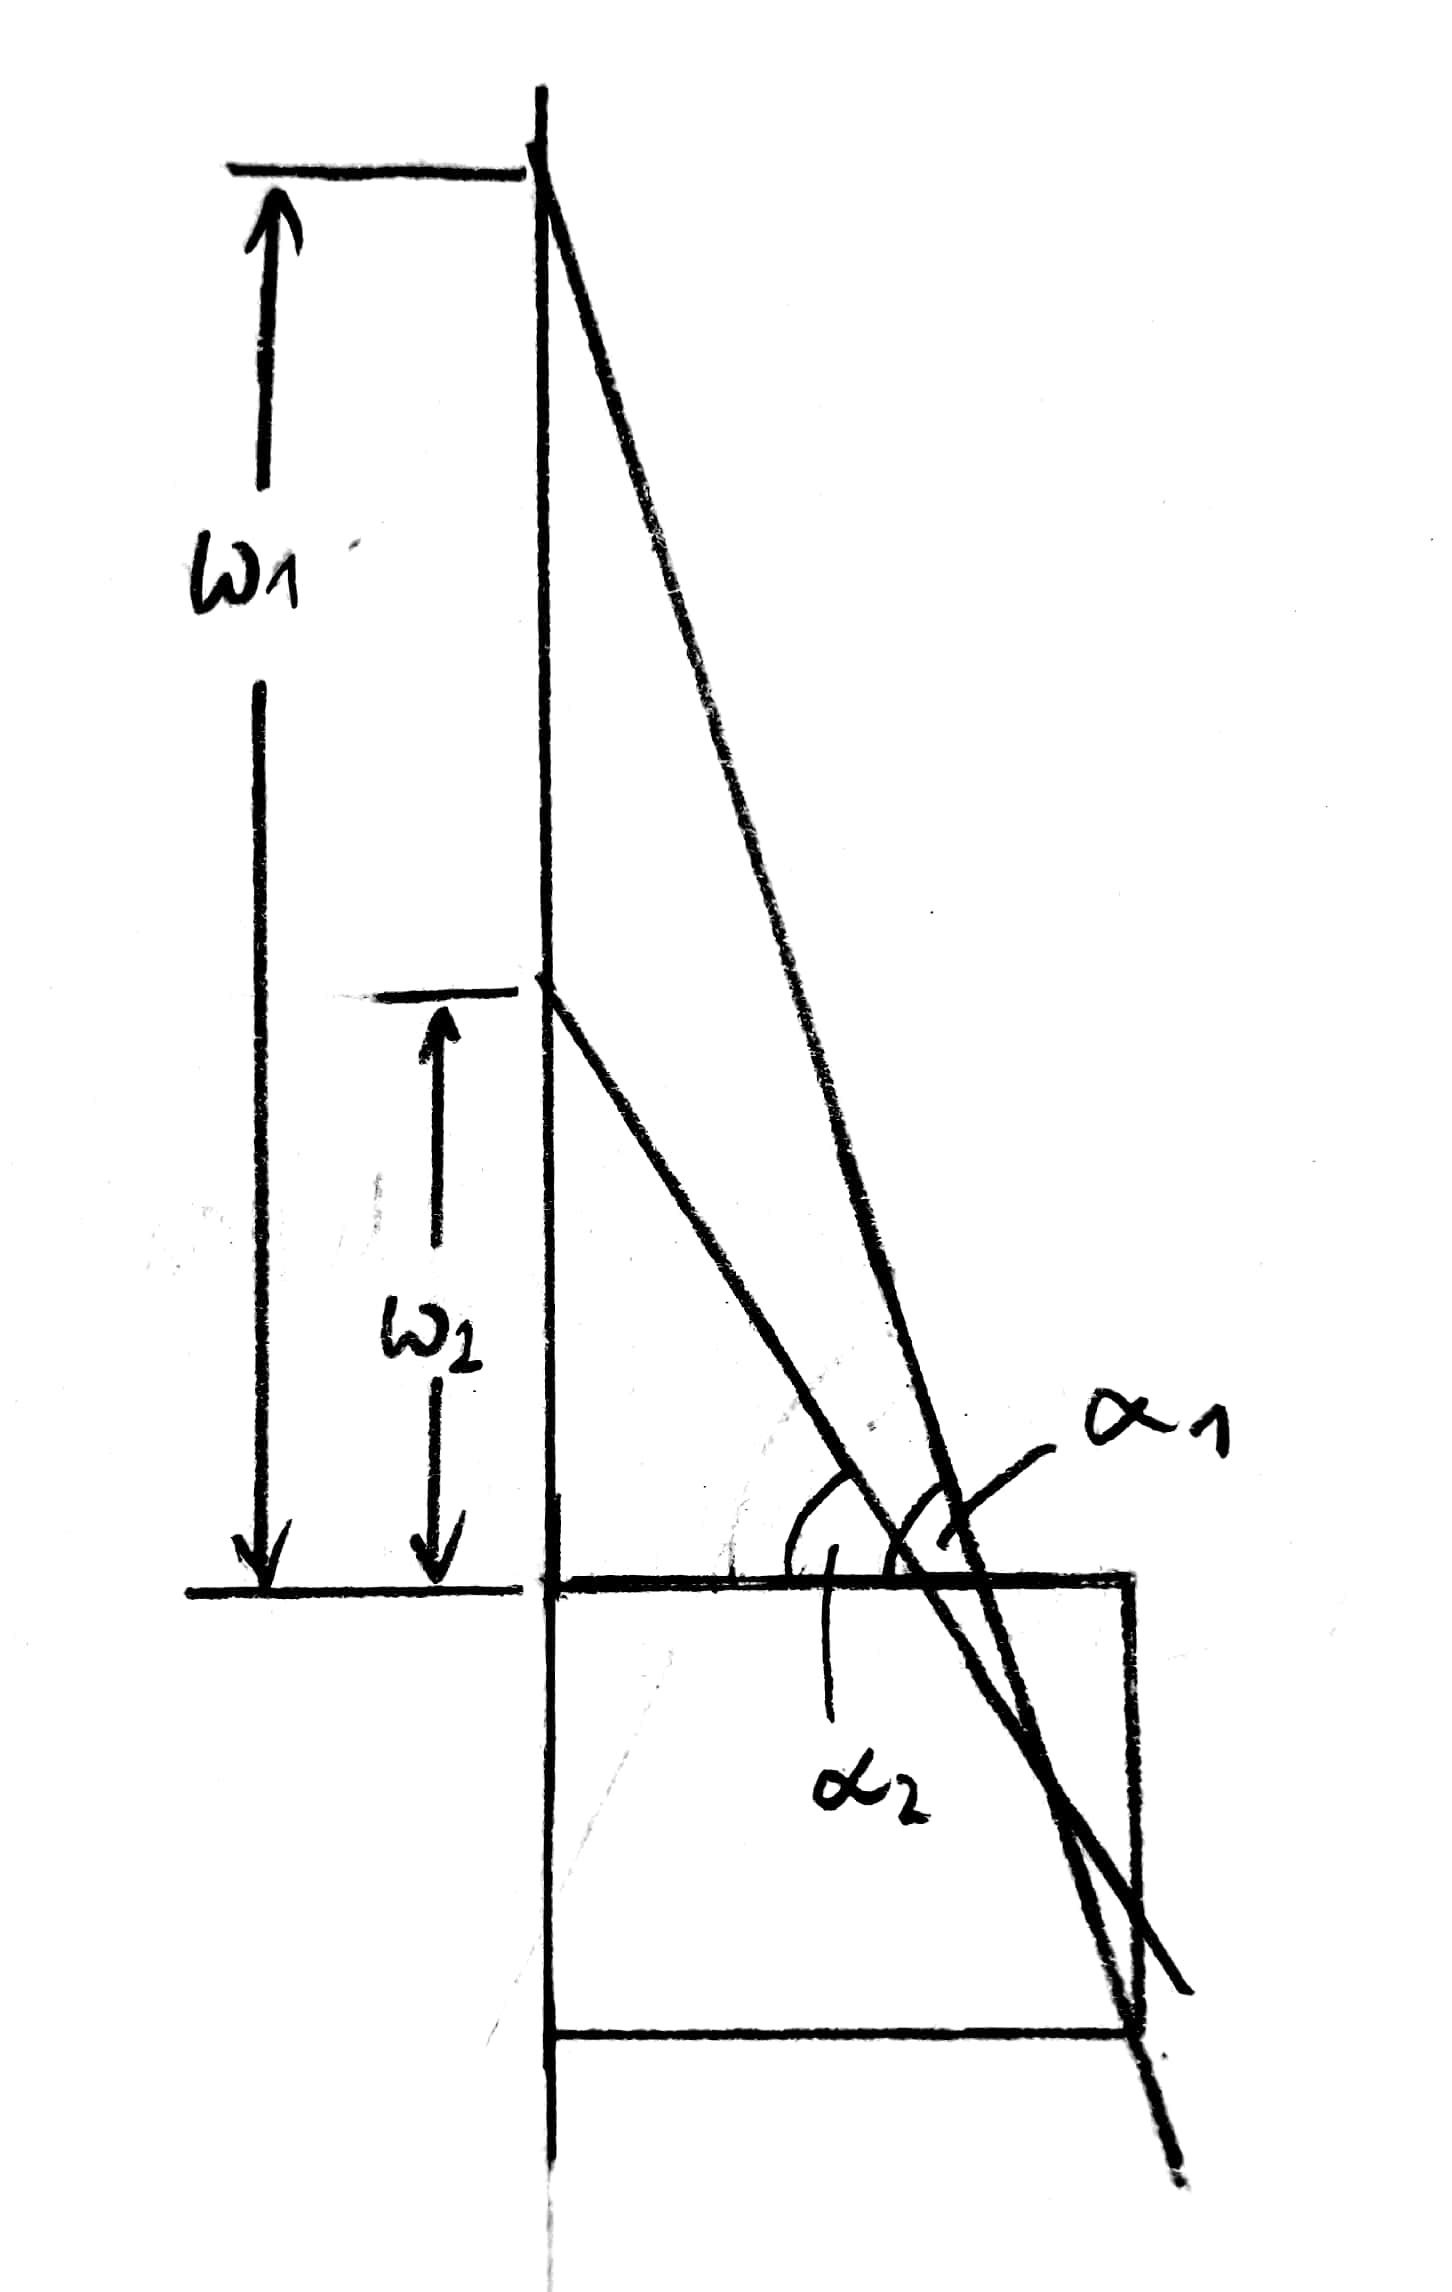
\includegraphics[width=.3\linewidth]{images/alpha_omega2.jpg}
		\caption{Problematik bei dieser Form der Geradenrepräsentation}
		\label{fig:alpha_omega2}
	\end{figure}

	Daher wurden für die beiden Geraden zwei verschiedene Repräsentationsformen gewählt. Für die linke ist der Offset als Schnittpunkt mit dem Linken Bildrand definiert, für die rechte Gerade ist es der Schnittpunkt mit dem rechten Bildrand. Die Winkel werden wie gehabt zur x-Achse gemessen. Die Umformung von der $\rho$-$\theta$-Form geschieht in der Funktion get\_offset\_alpha2 durch folgende Berechnungen: \\
	
	\begin{align*}
	\alpha=90^{\circ}-\theta
	\end{align*}
	
	
	Für Winkel $\theta<90^\circ$ (linke Fahrbahnlinie):
	
	\begin{align*}
	\omega&=-\frac{\rho}{\cos{90^{\circ}-\theta}} \\
	\end{align*}
	
	Für Winkel $\theta>90^\circ$ (rechte Fahrbahnlinie):
	
	\begin{align*}
	\omega&=\frac{B+\frac{\rho}{\cos{\theta-90^{\circ}}}}{\tan{90^{\circ}-\theta}} \\
	\end{align*}
	
	Mit der Bildbreite B.
	
	Abbildung \ref{fig:alpha_omega3} veranschaulicht diese Repräsentationsform.
	
	\begin{figure}[H]
		\centering
		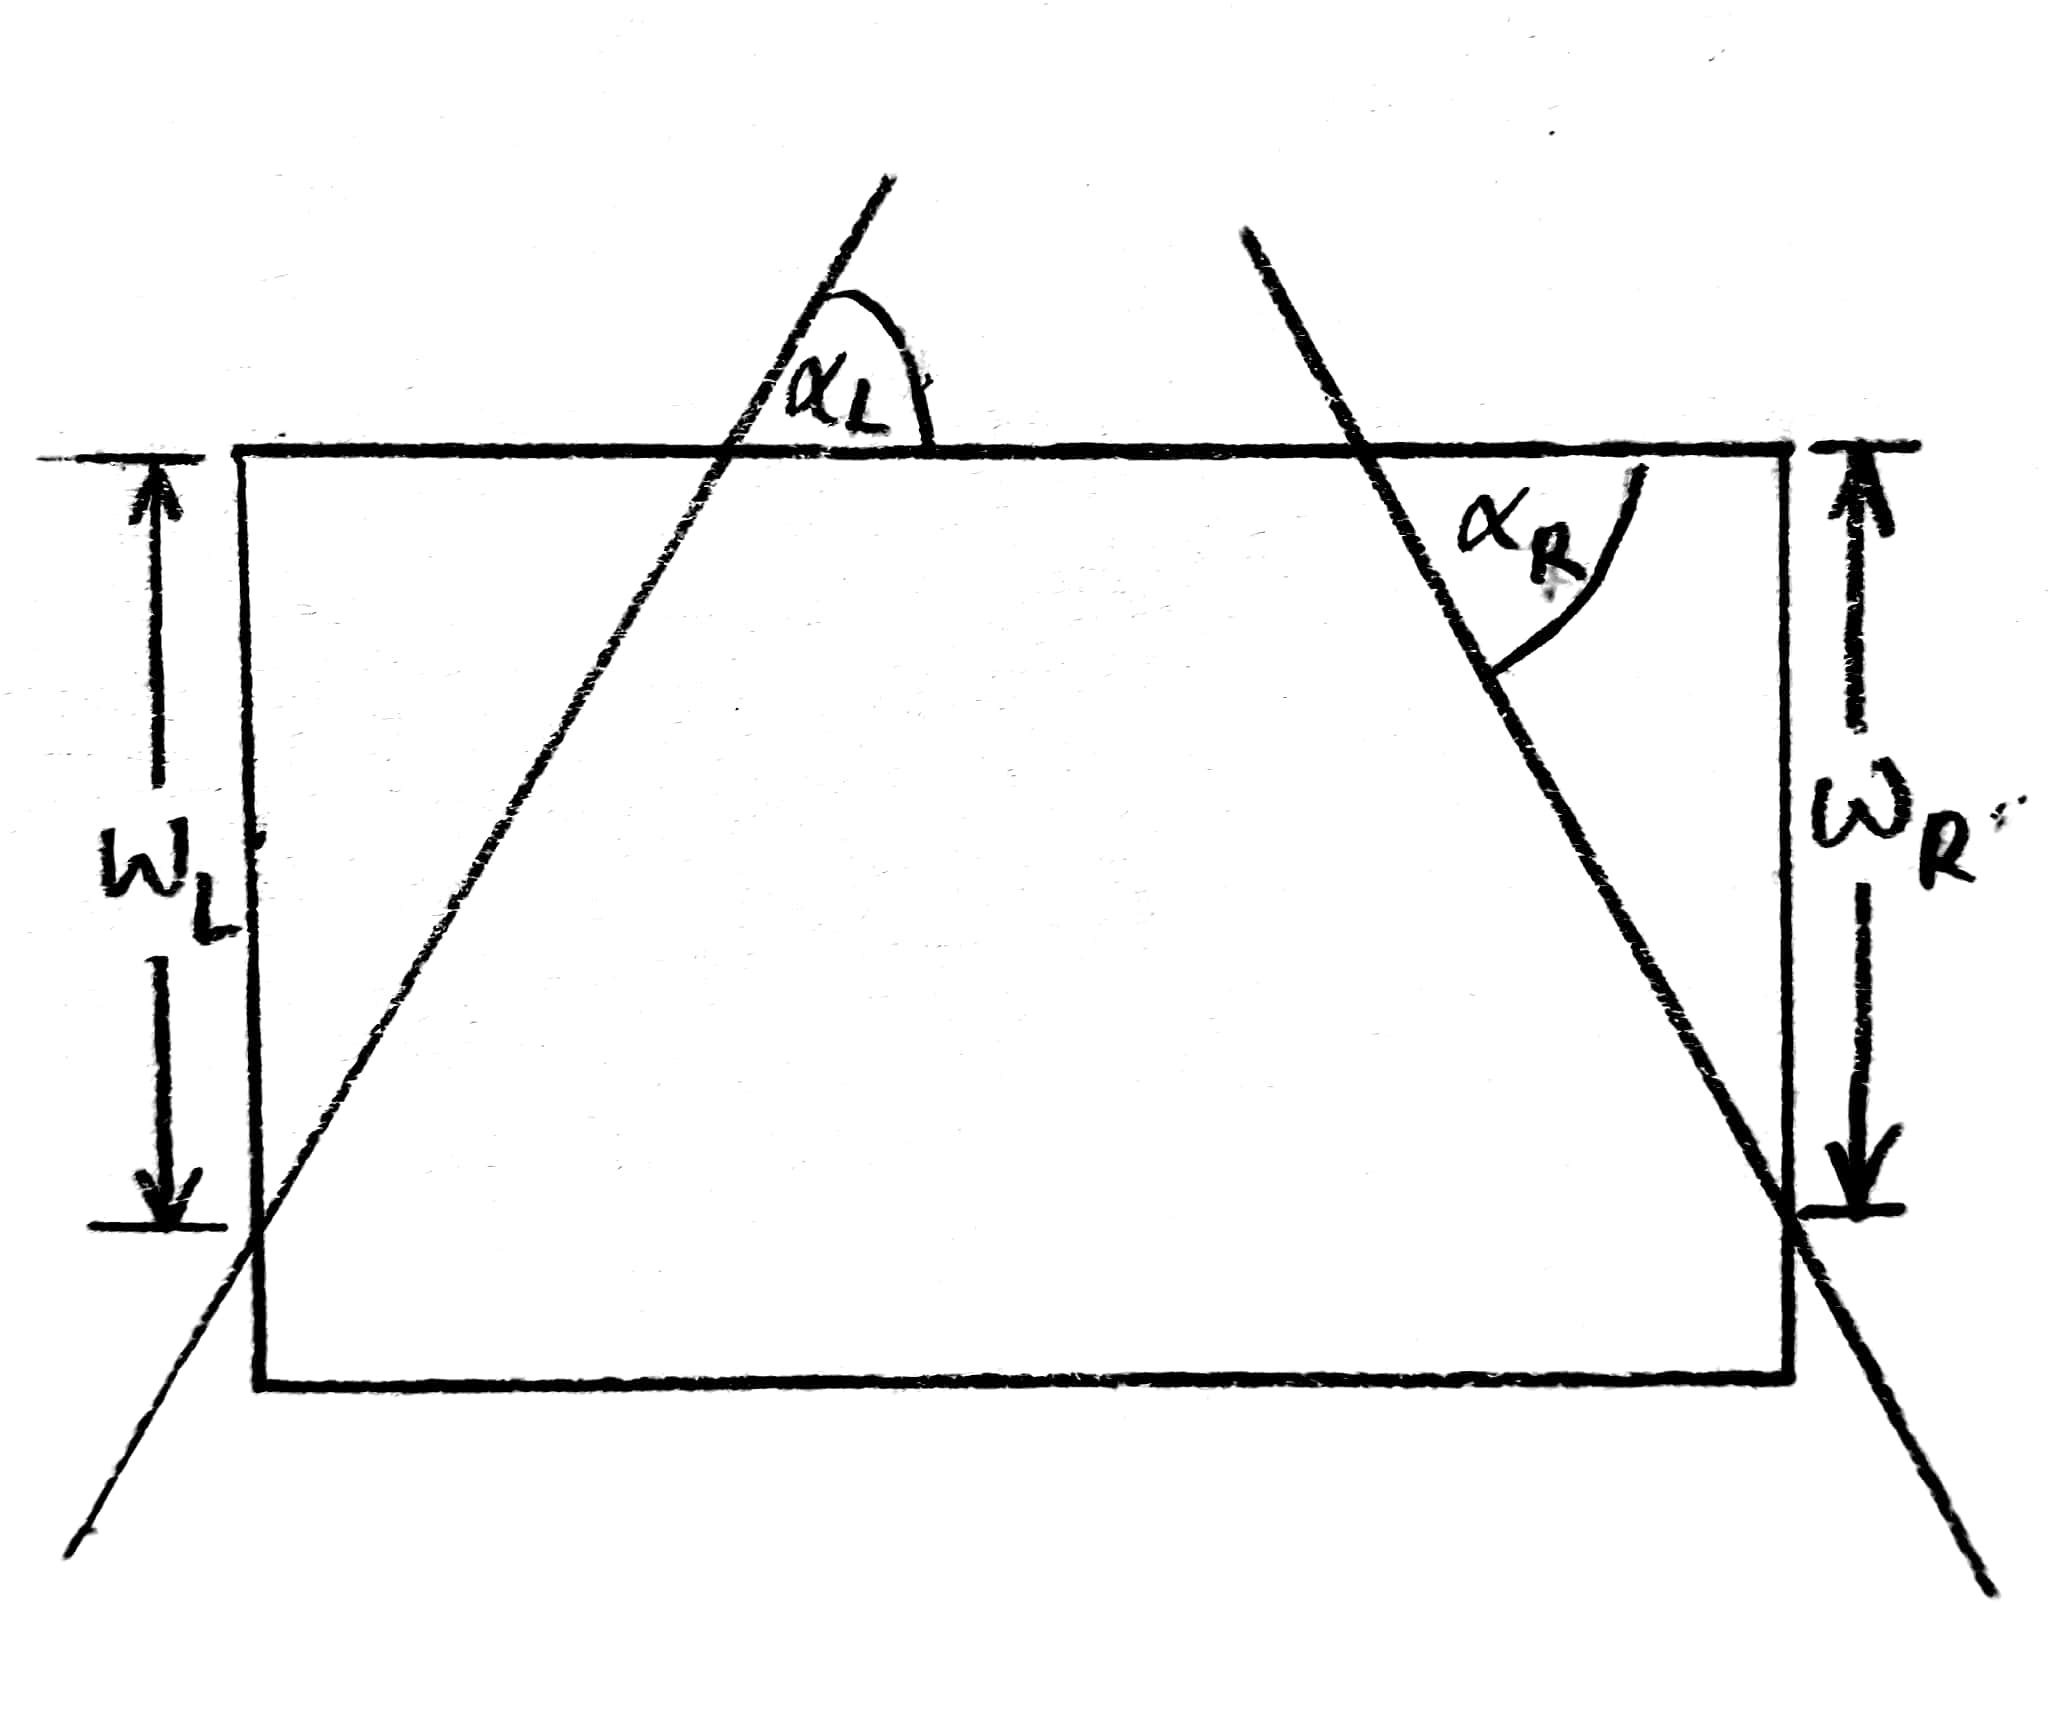
\includegraphics[width=.5\linewidth]{images/alpha_omega3.jpg}
		\caption{Beispiel für die Geradenrepräsentation durch Winkel $\alpha$ und Offsets $\omega$ gemessen von der linken und rechten oberen Ecke}
		\label{fig:alpha_omega3}
	\end{figure}


	Auch bei dieser Repräsentationsform könnten sich Problematische Fälle ergeben. Es wurde jedoch festgestellt, dass diese Form bisher am besten funktioniert.\\
	
	Alternativ wäre es möglich, die Geradenfindung nicht iterativ durchzuführen, und somit keinen Vergleich zwischen alten und neuen Gefundenen geraden durchführen zu müssen. Dazu müsste die Kamera so steil nach unten ausgerichtet werden, dass garantiert wird, dass nur die beiden Fahrbahnlinien erkannt werden, und keine anderen Linien.


	\subsection{Berechnung des Schnittpunktes der beiden Geraden}
	
	Der Lenkwinkel wird mithilfe der x-Koordinate des Fluchtpunktes, also des Schnittpunktes der beiden Geraden berechnet. Die Abweichung dieses x-Wertes vom Mittelpunkt wurde als Regeldifferenz verwendet.\\
	Die x-Koordinate des Fluchtpunktes (engl. vanishing point) wird in der Funktion get\_vp mit folgender Formel berechnet:\\
	
	\begin{align*}
	vp_x=\frac{\omega_R-\omega_L}{\tan{\alpha_L}+\tan{\alpha_R}} \\
	\end{align*}
	
	Um die Abweichung vom x-Wert der Bildmitte zu erhalten, wird von diesem Wert die Hälfte der Bildbreite B abgezogen:\\
	
	\begin{align*}
	\Delta x=vp_x-\frac{B}{2} \\
	\end{align*}
	
	
	\begin{figure}[H]
		\centering
		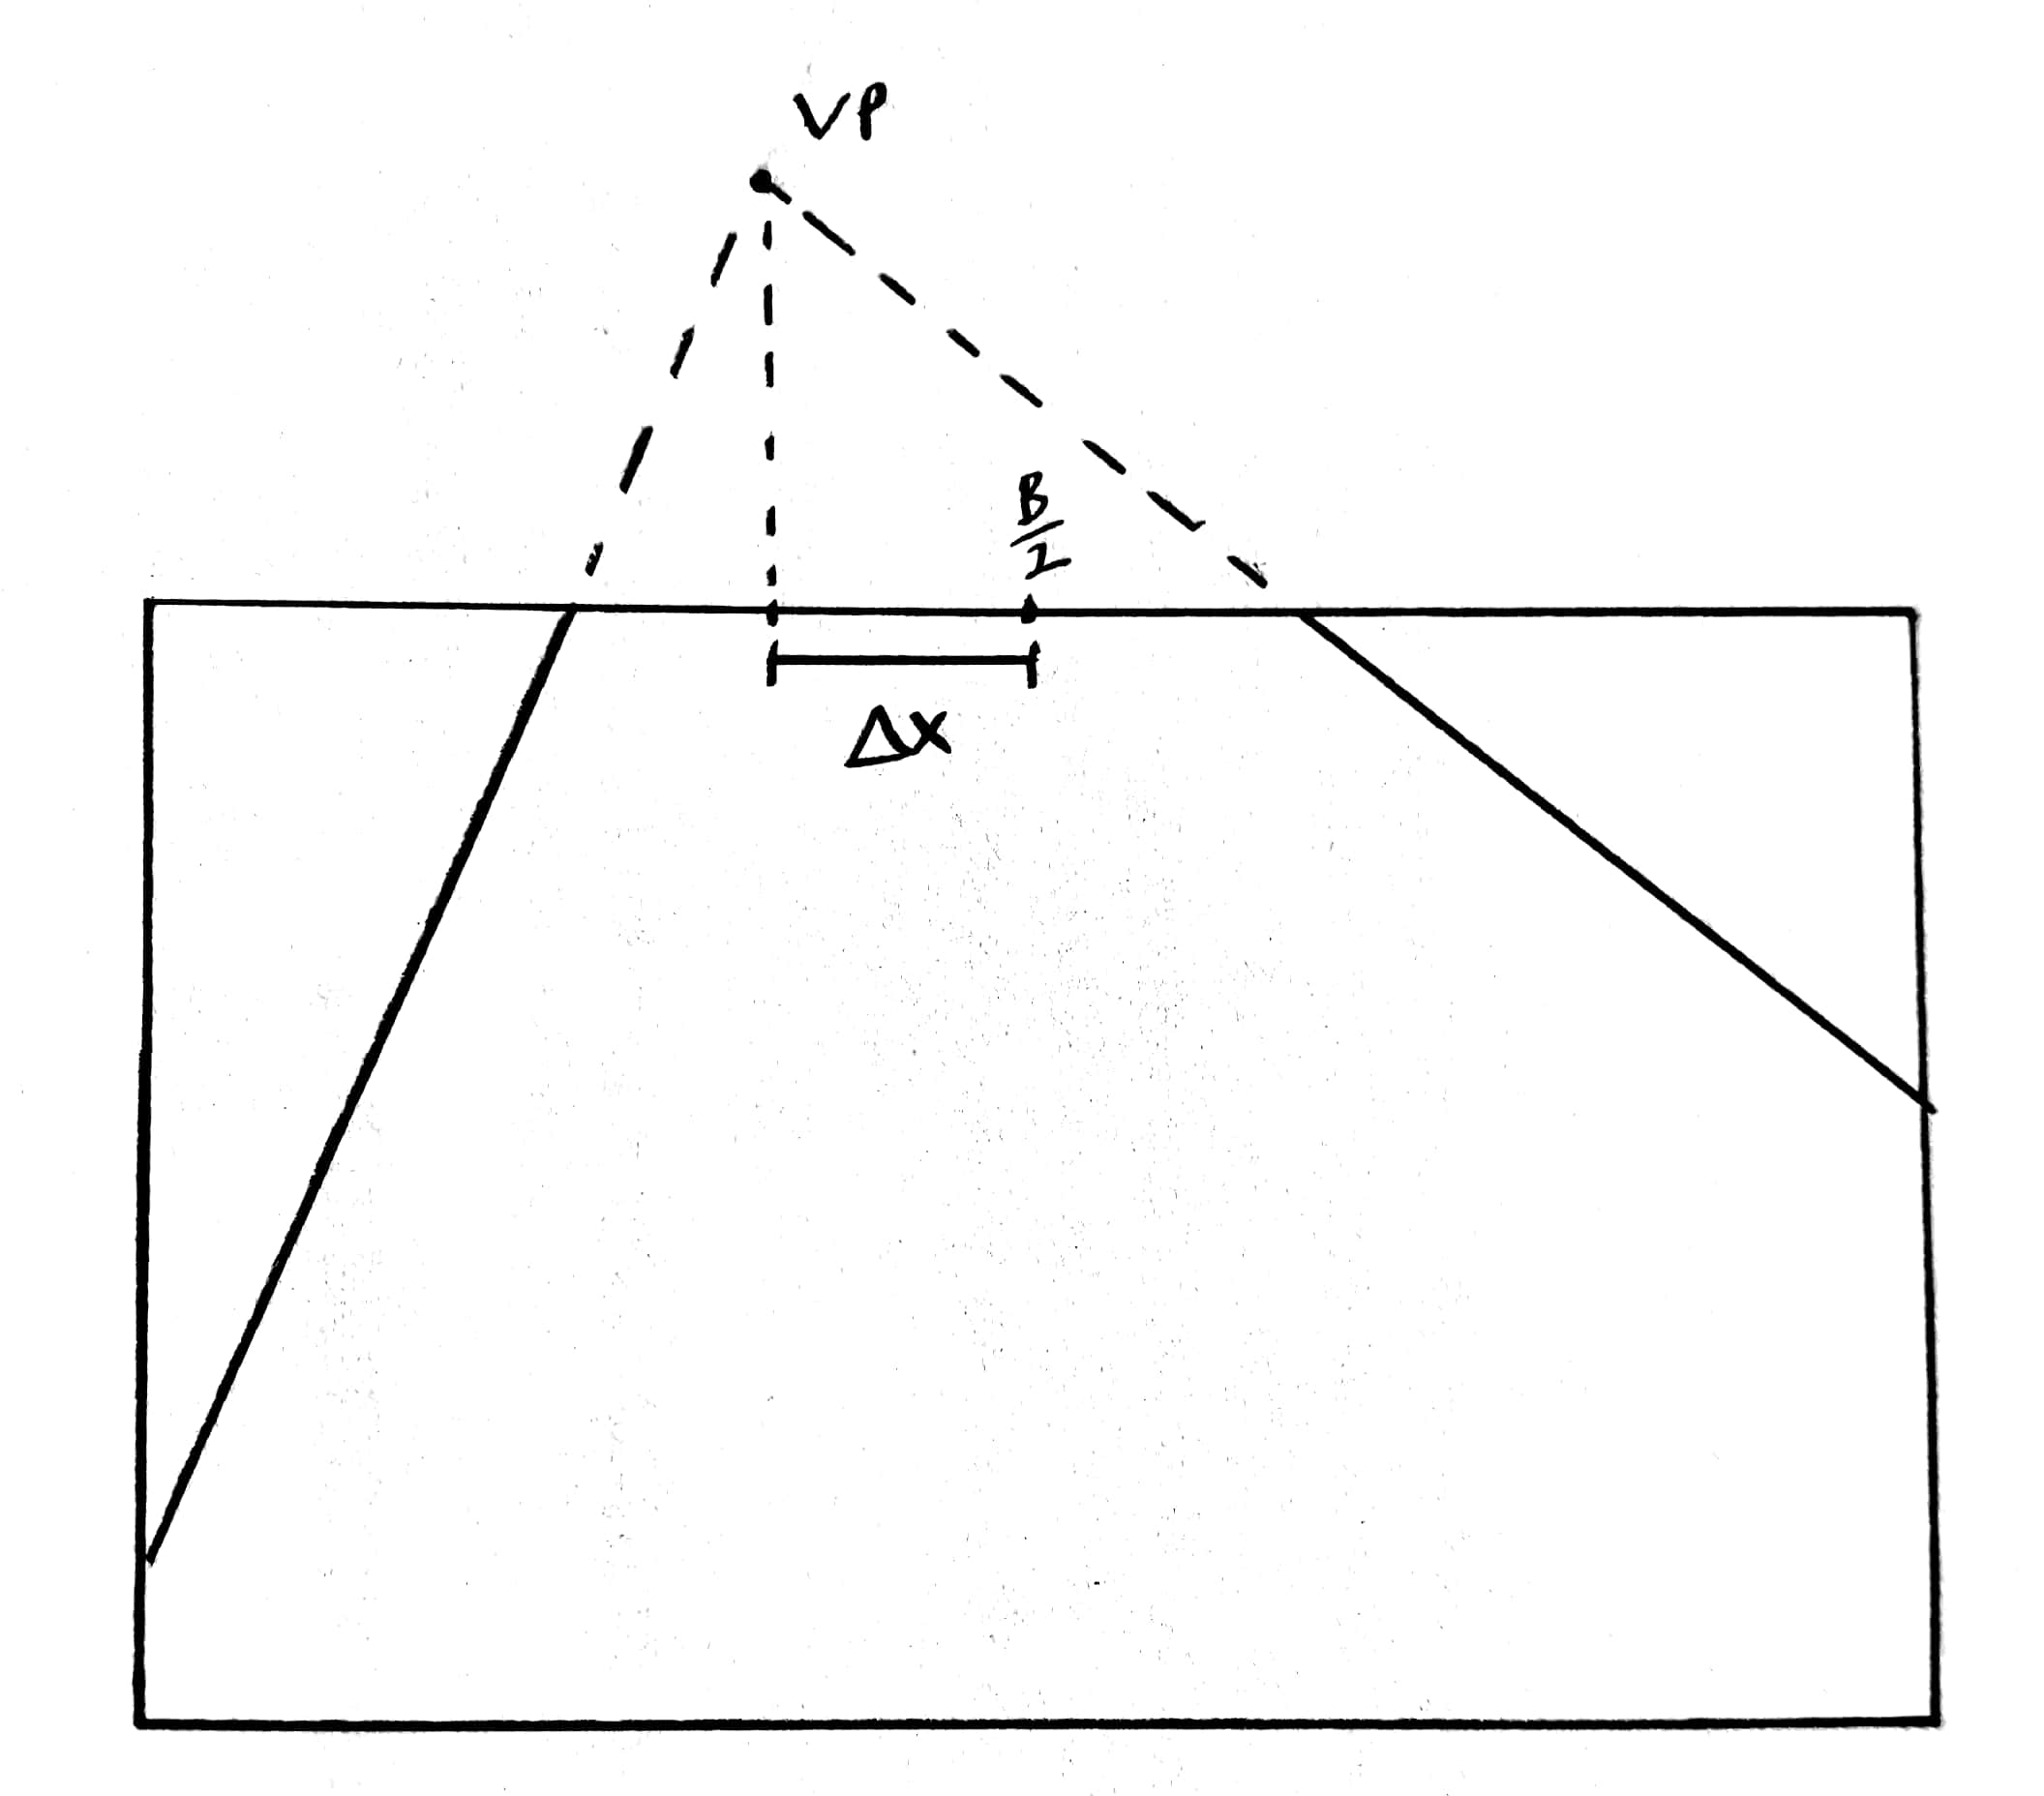
\includegraphics[width=.5\linewidth]{images/vp.jpg}
		\caption{Regeldifferenz als Differenz zwischen Bildmitte und x-Koordinate des Fluchtpunktes}
		\label{fig:alpha_omega3}
	\end{figure}

	Im Nachhinein wurde jedoch festgestellt, dass die Lage des Fluchtpunktes allein nicht ausreichend für die Steuerung des Wagen ist, da diese durch zwei Variablen definiert wird: Die horizontale Lage des Wagens auf der Fahrbahn (links, rechts) und seine Ausrichtung. So kann der Fluchtpunkt z.B. nach links verschoben sein, wenn der Wagen nah an der linken Fahrbahnlinie ist aber geradeaus fährt, oder aber wenn er mittig auf der Fahrbahn ist, aber nach rechts fährt. In beiden Situationen ist jedoch genau das umgekehrte Verhalten notwendig.
	
	\begin{itemize}
		\item Wagen nah an linker Fahrbahnlinie: nach rechts lenken
		\item Wagen mittig aber nach rechts ausgerichtet: nach links lenken
	\end{itemize}

	Es sind also noch mehr Kriterien einzubeziehen um den Wagen erfolgreich auf der Fahrbahn zu halten. Dabei besteht die Schwierigkeit darin, wie die verschiedenen Informationen (z.B. die beiden Winkel und Offsets der Linien) miteinander verrechnet werden, um am Ende eine Größe zu erhalten, die als Regelgröße verwendet werden kann. 
	
	
	
	
  
  \section{Ansteuerung von Servo und Motorcontroller}


Motorcontroller und Servo werden mithilfe eines Adafruit PCA9685 16-Kanal Servo Treibers angesteuert. Dieser nimmt Befehle des Raspberry Pi's über $I^2C$ entgegen und wandelt sie in ein PWM-Signal um. Das PWM Signal hat eine Periodendauer von 20ms, die Einschaltdauer $T_{on}$ liegt zwischen 1ms und 2ms. \\
Der Servotreiber hat eine eigene Bibliothek aus der am wichtigsten die Funktion set\_pwm(kanal, on,off) ist. Als Kanal wurde für den Servo 0 gewählt, für den Motorcontroller 1. Der Einschaltzeitpunt ''on'' wird immer auf 0 gesetzt. Für den Auschaltzeitpunkt kann theoretisch eine Zahl zwischen 0 und 4095 gesetzt werden. Da beim Servo das On-Signal zwischen einer und zwei Millisekunden lang sein muss ergibt sich der theoretische Wert folgendermaßen: \\

\begin{align*}
	off&=T_{on}\cdot\frac{20ms}{4096}\\
	off_{min}&=1ms\cdot\frac{20ms}{4096} =204,8\\
	off_{max}&=2ms\cdot\frac{20ms}{4096} = 409,6
\end{align*}

Für das verwendete Auto wurde der Min- und Maxwert empirisch ermittelt indem die geschaut wurde, bei welchen Werten die Räder bis zum Anschlag ausgelenkt sind. Es wurden folgende Werte ermittelt:\\

\begin{itemize}
	\item Vollausschlag rechts: 272
	\item Vollausschlag rechts: 342
	\item Mittelposition: 307
\end{itemize}

Als geeigneter Ausschlag nach rechts und links wurden die Werte 297 und 317 verwendet, damit nicht zu scharfe gelenkt wird.\\

Ebenso wurden für den Motor die Werte für den off-Parameter durch Ausprobieren ermittelt, indem geschaut wurde, bei welchen Werten das Auto mit angemessener Geschwindigkeit fährt. Hier wurden ermittelt:\\

\begin{itemize}
	\item Vorwärts: 320
	\item Rückwärts: 295
	\item Stop: 307
\end{itemize}


Die Funktion sendCommand(command) aus dem Modul modAct.py nimmt eine einen ganzzahligen Wert ''command'' entgegen, und sendet daraufhin mit set\_pwm ein PWM-Signal an den Servo oder Motorcontroller. Für vorwärts, rückwärts, stop, links, rechts und mitte wurden verschiedene Werte vorbelegt, mit bei denen set\_pwm mit den oben aufgelisteten Parametern aufgerufen wird. In diesen Fällen funktioniert die Steuerung diskret und es können nur drei feste Winkel und drei feste Motordrehzahlen eingestellt werden.\\
Ebenso kann sendCommand mit der einer Regeldifferenz, z.B. der Verschiebung des Fluchpunktes in x-Richtung, aufgerufen werden. Diese wird im aktuellen Programm direkt als Parameter der Funktion set\_pwm übergeben. In zukünftigen Projekten könnte man diese aber auch mit einer Konstanten multiplizieren, integrieren oder differenzieren um einen P-, PI- oder PID Regler zu implementieren.


	
	
	
	
	
	
%	Beim Start des Programms werden für die beiden Geraden feste Werte vorgegeben. Anhand dieser Anfangswerte werden die im nächsten Durchlauf die Fahrbahnlinien durch bessere Werte angenähert.\\
%	Dafür wird das Bild zunächst mithilfe eines Schwellwertes in Schwarzweiß umgewandelt. Bei einem geeigneten Schwellwert sollten nun möglichst nur die beiden Fahrbahnlinien weiß sein (den Wert 1 haben).\\
%	Als nächstes wird die Funktion HoughLines aus der Bibliothek cv ausgeführt, die alle Geraden im Bild sucht. Die Funktion Houghlines gibt als Rückgabewert eine Liste von Geraden zurück, die in Polarkoordinaten durch einen Winkel $\rho$ und ein Abstand $\theta$ repräsentiert werden. $\rho$ ist der Winkel zwischen der Normalen, die senkrecht auf der Geraden steht, und der x-Achse. $\theta$ ist die Länge dieser Normalen, d.h. der Abstand zwischen der Geraden und dem Ursprung des Koordinatensystems.
	
 
	
	

  % \bibliography{hawey-documentation}
  % \bibliographystyle{ieeetr}

  % Bibliograpy / Literaturverzeichnis
  \newpage
  %\bibliography{literatur}
  \addcontentsline{toc}{section}{Literaturverzeichnis}
  % display bibliography
 
\end{document}
